\documentclass[10pt,a4paper,openright]{report}


\usepackage[width=15.00cm, height=25.00cm]{geometry}
\usepackage[italian]{babel}
\usepackage[utf8]{inputenc}
\usepackage[T1]{fontenc}
\usepackage{dsfont}
\usepackage{amsmath}
\usepackage{amsfonts}
\usepackage{amssymb}
\usepackage{graphicx}
\usepackage{paracol}
\usepackage{xparse}
\usepackage{sidecap}
\usepackage[makeroom]{cancel}
\usepackage{capt-of}
\usepackage{caption}
\usepackage[dvipsnames]{xcolor}
\usepackage{xpatch}
\usepackage{subcaption}
\usepackage[most]{tcolorbox}
\usepackage{lipsum}
\usepackage{float}
\usepackage{imakeidx}
\usepackage{wrapfig}
\usepackage[shortlabels]{enumitem}
\usepackage{marginnote}
\usepackage{tickzit}
\usepackage{bm}
\usepackage{textcomp}
%\usepackage{enumerate}

\input{stilifigure.tikzstyles}
%\makeindex[columns=3, title=Indice Analitico, intoc]


\graphicspath{{Immagini/}}
\setcolumnwidth{0.3\textwidth}

\captionsetup{font = {it, small}, labelfont={color=NavyBlue, bf}}


\newcommand{\four}[1]{\mathfrak F \left(#1\right)}
\newcommand{\antif}[1]{\mathfrak F^{-1} \left(#1\right)}
\newcommand{\ov}{\boldsymbol}
\newcommand{\med}{\textrm{med}}
\newcommand{\rng}{\textrm{rng}}
\newcommand{\cov}{\textrm{cov}}
\newcommand{\pval}{p\textrm{-value}}
\newcommand{\vett}[1]{\boldsymbol{#1}}




















\newcommand{\de}[1]{\textbf{\textcolor{NavyBlue}{#1}}}
\newcommand{\figura}[5]{\begin{SCfigure}[#2][b!h!t!]
		\centering
		\includegraphics[width=#1 cm]{#3}
		\caption{#4} \label{#5}
\end{SCfigure}}

\newcommand{\pd}[2]{\frac{\partial #1}{\partial #2}}


\newcounter{concetti}
\newenvironment{concetto}{
	\refstepcounter{concetti}
	{\color{NavyBlue}\textbf{Concetto \theconcetti:}} \quad
}{
	
}
\numberwithin{concetti}{chapter}
\tcolorboxenvironment{concetto}{
	boxrule=0pt,
	boxsep=0pt,
	colback={White!90!NavyBlue},
	enhanced jigsaw, 
	borderline west={2pt}{0pt}{NavyBlue},
	sharp corners,
	before skip=5pt,
	after skip=10pt,
	breakable,
}


\newenvironment{dimostrazione}{
	\noindent
	{\color{YellowGreen}\textbf{Dimostrazione:}}
}{
}
\tcolorboxenvironment{dimostrazione}{
	boxrule=0pt,
	boxsep=0pt,
	colback={White!100!YellowGreen},
	enhanced jigsaw, 
	borderline west={2pt}{0pt}{YellowGreen},
	sharp corners,
	before skip=5pt,
	after skip=5pt,
	breakable,
}

\newcounter{numnote}
\numberwithin{numnote}{chapter}
\newenvironment{nota}{
	\noindent
	\refstepcounter{numnote}
	{\color{YellowGreen}\textbf{Nota \thenumnote:}}
}{
}
\tcolorboxenvironment{nota}{
	boxrule=0pt,
	boxsep=0pt,
	colback={White!90!YellowGreen},
	enhanced jigsaw, 
	borderline west={2pt}{0pt}{YellowGreen},
	sharp corners,
	before skip=5pt,
	after skip=5pt,
	breakable,
}


\newcounter{numrichiamo}
\numberwithin{numrichiamo}{chapter}
\newenvironment{richiamo}{
	\noindent
	\refstepcounter{numrichiamo}
	{\color{ForestGreen}\textbf{Richiamo \thenumrichiamo:}}
}{
}
\tcolorboxenvironment{richiamo}{
	boxrule=0pt,
	boxsep=0pt,
	colback={White!90!ForestGreen},
	enhanced jigsaw, 
	borderline west={2pt}{0pt}{ForestGreen},
	sharp corners,
	before skip=5pt,
	after skip=5pt,
	breakable,
}

\newcounter{esempi}
\numberwithin{esempi}{chapter}
\newenvironment{esempio}[1]{
	\noindent
	\refstepcounter{esempi}
	{\color{Periwinkle}\textbf{Esempio \theesempi#1} \\ } 
	
	
	\noindent
	\renewcommand{\de}[1]{\textbf{\textcolor{Periwinkle}{#1}}}
}{
}


\tcolorboxenvironment{esempio}{
	boxrule=0pt,
	boxsep=0pt,
	colback={White!90!Periwinkle},
	enhanced jigsaw, 
	borderline west={2pt}{0pt}{Periwinkle},
	sharp corners,
	before skip=10pt,
	after skip=10pt,
	breakable,
}











\title{Sistemi Meccanici e Modelli \\ Prof.: Mauro Da Lio}
\author{Matteo Dalle Vedove}
\date{Anno Accademico 2020-2021 \\ \today}



\begin{document}
	\pagenumbering{roman}
	
	\begin{center}
		\vspace{3cm}
		\thispagestyle{empty}
		
\includegraphics[width=5cm]{logouni}
		
		\vspace{2cm}
		
		{\Large Università degli Studi di Trento}
		
		\vspace{2cm}
		{\Large Dipartimento di Ingegneria Industriale} \\ \vspace{2mm}
		{\LARGE \textbf{Corso di Misure Meccaniche e Termiche}} \\ \vspace{2mm}
		{\Large Docente: De Cecco Mariolino}\\
		
		\vspace{2cm}
		{\LARGE \textbf{Appunti del corso}}
		
		\vspace{2cm}
		{\large 
			Matteo Dalle Vedove \\
			\makeatletter
			matteo.dallevedove@studenti.unitn.it
			
			\vspace{2cm}
			Anno Accademico 2020-2021 \\ 28 gennaio 2021}
	\end{center}
	
	\tableofcontents
	
	
	\pagenumbering{arabic}
	
	
	\chapter{Introduzione}
	\de{Misurare}
	
	
	
\section{Teoria generalizzata degli strumenti di misura}
	Gli \de{elementi funzionali} individualibili un un apparato (o sistema) di misura:
	\begin{enumerate}
		\item il \textbf{sensore primario}: l'elemento sensibile al misurando. E' l'elemento in diretto contatto con il misurando (o è preceduto da un elemento trasmettitore). Esso riceve energia dal misurando e, a volte, può effettuare una trasformazione di variabile. In generale è importante che questo sensore perturbi il meno possibile il misurando, assorbendo il minimo di energia;
		
		\item l'\textbf{elemento di trasmissione}: è un elemento un cui la grandezza di ingresso è pari a quella in uscita ma opera una trasduzione di posizione del segnale utile. In particolare esso deve attenuare, distorcere e ritardare il meno possibile il segnale condotto;
		
		\item l'\textbf{elemento di conversione di grandezza} o \textbf{trasformatore di variabile}: è utilizzato per facilitare la trasmissione del segnale a distanza. Può anche essere utilizzato per elaborare il segnale (come amplificarlo o filtrarlo). In generale si ha la trasformazione in questo punto in grandezze elettriche;
		
		\item\textbf{ elemento di elaborazione dati}: utilizzato per elaborare i dati come la codifica dei segnali per la trasmissione, per amplificare ulteriormente i segnali, estrarre informazioni aggiuntive o ridurre l'effetto degli ingressi di disturbo. Si ha elaborazione anche quando si integra/deriva una variabile per ottenere informazioni ulteriori o convertire segnali da analogico a digitale (e viceversa);
		
		\item \textbf{elemento di memorizzazione}: servono a memorizzare (a breve o lungo termine) le informazioni provenienti da un sistema di misura. Essi permettono di cambiare anche la scala dei tempi di riproduzione dei dati;
		
		\item \textbf{elemento di presentazione dati}: fornisce l'uscita dei dati in una forma reattiva ai sensi dell'uomo (tendenzialmente segnali visivi).
	\end{enumerate}	
	
	\chapter{Misure di deformazione mediante estensimetri}

\section{Cenni sullo stato di tensione piano e triassiale}
	Considerando uno \de{stato di tensione piano} (tensione perpendicolare al piano $\sigma_z=0$), è possibile determinare le deformazioni $\epsilon_x, \epsilon_y$ lungo gli assi $x$ e $y$ rispettivamente supponendo di conoscere le tensioni $\sigma_x,\sigma_y$ lungo gli stessi. Noto il \de{modulo di Young} $E$ e il \de{coefficiente di Poisson} $\nu$ si verifica infatti che
	\begin{equation} \label{eq:def:defpiana}
		\epsilon_x = \frac{\sigma_x}{E} - \nu \frac{\sigma_y}{E} \qquad \epsilon_y = \frac{\sigma_y}{E} - \nu \frac{\sigma_x}{E}
	\end{equation}
	
	Le deformazioni $\epsilon$ rappresentano una variazione di lunghezza $\Delta L$ riferite ad una lunghezza $L$, e in generale si considera
	\[ \epsilon = \frac{\Delta L}{L} \qquad \left[\frac {\mu m} m \right]\]
	
	Invertendo opportunamente le formule è possibile determinare le tensioni $\sigma_i$ lungo i vari assi del piano come
	\[ \sigma_x = \frac{E \big(\epsilon_x + \nu \epsilon_y \big)}{1-\nu^2} \qquad \sigma_y = \frac{E \big(\epsilon_y + \nu \epsilon_x \big)}{1-\nu^2} \]
	
	\paragraph{Stato di tensione triassiale} Estendendo i concetti della deformazione di uno stato piano allo spazio, è possibile definire la deformazione $\epsilon$ lungo gli assi nello spazio riprendendo l'equazione \ref{eq:def:defpiana} riscritta come
	\begin{equation}
		\epsilon_x = \frac{\sigma_x}{E} - \nu \frac{\sigma_y}{E} - \nu \frac{\sigma_z}{E} \qquad \epsilon_y = \frac{\sigma_y}{E} - \nu \frac{\sigma_x}{E} - \nu \frac{\sigma_z}{E} \qquad \epsilon_z = \frac{\sigma_z}{E} - \nu \frac{\sigma_x}{E} - \nu \frac{\sigma_y}{E}
	\end{equation}

\section{Classificazione degli estensimetri}
	Gli \de{estensimetri} sono utilizzati per determinare deformazioni superficiali locali (quindi analizzando punti molto vicini tra loro). Sono detti invece \de{estensometri} i componenti atti a determinare deformazioni medie superficiali su punti \textit{distanti} tra loro.
	
	Gli estensimetri possono essere:
	\begin{itemize}
		\item meccanici, i più antichi. Sono composti da due coltelli (uno fisso e uno mobile) che tramite delle leve meccaniche permettono di amplificare il loro spostamento relativo permettendo di visualizzare con precisione l'estensione dei punti oggetti di studio;
		
		\item acustici;
		\item ottici;
		\item elettrici a resistenza; comunemente i più usati attualmente.
	\end{itemize}

\section{Estensimetro a resistenza elettrica}
	\subsection*{Caratteristiche desiderate}
		Le caratteristiche desiderate in ogni estensimetro sono:
		\begin{itemize}
			\item che la costante di taratura sia stabile e tempo invariante, sia per effetti termici che altri fattori ambientali;
			\item deve misurare la deformazione locale e non quella media, quindi deve riuscire ad analizzare punti molto vicini tra loro;
			\item deve avere  una buona risposta in frequenza per rilevare deformazioni che avvengono molto velocemente;
			\item devono essere economicamente accessibili per favorire un largo impiego.
		\end{itemize}
	
	\subsection{Principio di funzionamento}
		Il funzionamento di un estensimetro a resistenza $R$ si basa sul fatto che tale proprietà risulta essere proporzionale all'allungamento del filo rispetto alla quale è ricavato. In particolare disponendo un filo a maglia (quindi la lunghezza complessiva è elevata), applicando ai suoi terminali una tensione costante è possibile determinare la resistenza $R$ del circuito fortemente determinata dall'allungamento.
		
		Estensimetri elettrici presentano tendenzialmente resistenze interne pari a $R=120\Omega,350\Omega$. Ogni soluzione presenta dei vantaggi ma anche degli svantaggi, come si può osservare in tabella \ref{tab:def:vantaggi}. Questo tipo di estensimetri permettono di misurare punti inizialmente posti tra $0.6mm$ e $200mm$.
		
		\begin{SCtable}[0.5][b!]
			\centering
			\begin{tabular}{p{5cm} p{1.2cm} p{1.2cm} }
				 &   $120\Omega$ &  $350\Omega$ \\ \hline
				 corrente di alimentazione &   alta &   bassa \\ \hline
				 autoriscaldamento &   alto &   basso \\ \hline
				 sensibilità alla riduzione dell'isolamento &   bassa &   alta \\ \hline
				 sensibilità all'interferenza elettromagnetica &   bassa &   alta \\ \hline
				 effetto di resistenze nella trasmissione (cavi) &   alto &   basso \\
			\end{tabular}
			\caption{vantaggi e svantaggi associati alle resistenze iniziale degli estensimetri elettrici.} \label{tab:def:vantaggi}
		\end{SCtable}
		
	\subsubsection{Dimostrazioni matematiche}
		Per un conduttore filiforme di lunghezza $l$ e sezione $A$, allora la resistenza $R$ dello stesso è pari a 
		\begin{equation}
			R= \rho \frac l A
		\end{equation}
		dove $\rho$ è la \de{resistività} del materiale, ossia una proprietà intrinseca del metallo che compone il conduttore. Per determinare la variazione di resistenza $\delta R$ rispetto alla resistenza $R$ è necessario differenziare tale equazione, con il risultato che
		\begin{align*}
			\frac{\delta R}{R} & = \frac 1 R \left( \pd R \rho \delta \rho + \pd R l \delta l + \pd R A \delta A \right) \\ 
			& = \frac{\delta \rho}{\rho} + \frac{\delta l}{l} - \frac{\delta A}{A}
		\end{align*}		
		
		In generale l'area $A$ della sezione del filo può essere espressa, tramite un fattore di forma $C$ costante, come proporzionale al quadrato del diametro $d$ del conduttore, e dunque
		\[ A = C d^2 \qquad \rightarrow \frac{\delta A}{A} = \cancel{\pd A C\delta C}+ \pd A d \delta d = 2\frac{Cd \, \delta d}{A} = 2\frac{\delta d}{d}\]
		A questo punto la variazione della resistenza del conduttore può essere espressa come 
		\[ \frac{\delta R}{R} =  \frac{\delta \rho}{\rho} + \frac{\delta l}{l} - 2\frac{\delta d}{d} \]
		
		Nota la deformazione assiale $\epsilon_a$ (in quanto è quella che determina la misura di deformazione), allora ad essa è associata anche una deformazione trasversale $\epsilon_t = - \nu \epsilon_a$. Considerando che $\epsilon_a$ rappresenta il termine $\delta l/l$ l'espressione della resistenza può essere riscritta come:
		\begin{align*}
			\frac{\delta R}{R} =  \frac{\delta \rho}{\rho} + \frac{\delta l}{l} - 2\left( -\nu \frac{\delta l}{l} \right) & = \frac{\delta \rho}{\rho} + \frac{\delta l}{l} \big(1+2\nu\big) \\ 
			& = \epsilon_a \frac{\delta \rho}{\rho \epsilon_a} + \epsilon_a \big(1+2\nu\big) = \epsilon_a \left( \frac{\delta \rho}{\rho \epsilon_a} +  1+2\nu\right)
		\end{align*}
		
		\begin{concetto}
			A questo punto è possibile esprimere la \de{prima legge fondamentale dell'estensimetria} che permette di definire la \de{sensibilità dell'estensimetro} $K$:
			\begin{equation} \label{eq:def:primalegge}
				K = \frac{\delta R / R}{\epsilon_a} = \frac{\delta \rho}{\rho \epsilon_a} + 1 + 2\nu
			\end{equation} 
		\end{concetto} 
	
		Il termine $1+2\nu$ rappresenta la \de{sensibilità geometrica} ed è sempre un valore costante (essendo $\nu = 0.3$ per i metalli, allora essa vale circa $1.6$), mentre il termine $\delta \rho / \rho \epsilon_a$ rappresenta la \de{sensibilità piezoresistiva} (circa 0.4 per estensimetri metallici, tra 100 e 1000 per quelli a semiconduttore). Si osserva che questo secondo termine dipende esplicitamente dalla deformazione $\epsilon_a$, e dunque può essere trascurato per piccole deformazioni, ma può diventare importante per estensioni maggiori.
		
		Con questa legge è dunque possibile correlare resistenza elettrica ed estensione come
		\[ \frac {\delta R} R = K \epsilon_a  \]
		
		\paragraph{Sensibilità trasversale} Le relazioni appena indicate non considerano il fatto che gli estensimetri contengano tratti di griglia perpendicolari all'asse di misura che subiscono delle deformazioni differenti $\epsilon_t$. Tuttavia questi tratti sono pochi e di dimensioni limitati, e per questo spesso è convenienti trascurarli. 
		
		Considerando che la sezione trasversale ha una sensibilità $K_t$, è possibile determinare il \de{coefficiente di sensibilità trasversale} $S_t$ come segue che permette di ridefinire l'equazione di variazione di resistenza:
		\[ S_t = \frac{K_t}{K} \qquad \rightarrow \frac {\delta R} R = K\big(\epsilon_a+ S_t\epsilon_t\big)  \]
		
		Considerando che in generale $S_t < 1\%$ e che $\epsilon_t<\epsilon_a$, trascurando il termine dovuto alla sensibilità trasversale non comporterebbe l'introduzione di un errore significativo (per piccole deformazioni).
		
	\subsection{Lettura degli estensimetri}
	\subsubsection{Ponte di Wheatstone}
		Per interpretare le variazioni di resistenza degli estensimetri si ricorre all'utilizzo del \de{ponte di Wheatstone} (figura \ref{wheatstone}), un circuito particolare di elementi resistivi che permette di determinare lo \de{sbilanciamento} $e_0$ del ponte.
		
		\figura{5}{0.75}{wheatstone}{circuito del ponte di Wheatstone.}{wheatstone}
		
		Alimentando ad una tensione costante $E$ il circuito, tramite le equazioni di Kirchhoff è possibile determinare delle relazioni algebriche tra sbilanciamento $e_0$ e tensioni di alimentazione. Considerando il sistema di equazioni:
		\[ \begin{cases}
			-e_0 - R_2I_2 +R_1I_1 = 0 \\ E = (R_1+R_4) I_1 \\ E = (R_2+R_3)I_2
		\end{cases}\]
		e' possibile determinare il rapporto $e_0/E$ come:
		\[ \frac{e_0}{E} = \frac{R_1}{R_1+R_4} - \frac{R_2}{R_2+R_3} = \frac{R_1R_3-R_2R_4}{\big(R_1+R_4\big) \big(R_2+R_3\big)} \]
		
		Supponendo di avere il ponte inizialmente azzerato, allora deve valere che $e_0 = R_1R_3-R_2R_4=0$. Considerando che la resistenza $R_1$ vari di una quantità $\Delta R_1$ (assumendo valore complessivo $R_1+\Delta R_1$), allora è possibile (tramite la relazione mostrata precedentemente) determinare la variazione di sbilanciamento $\Delta e_0$ del ponte come:
		\begin{align*}
			\frac{\Delta e_0}{E} & = \frac{\big(R_1+\Delta R_1\big)R_3-R_2R_4} {\big(R_1+\Delta R_1+R_4\big)\big(R_2+R_3\big)} = \frac{\Delta R_1 R_3}{\big(R_1+R_4\big) \big(R_2+R_3\big) + \Delta R_1 \big(R_2+R_3\big)} \\
			 &= \frac{\Delta R_1 R_3}{\big(R_1+R_4\big) \big(R_2+R_3\big) } \frac{1}{1+\frac{\Delta R_1}{R_1+R_4}}
		\end{align*}
		
		Introducendo i parametri $\alpha= R_3 / (R_2+R_3)$ e $R_m = R_1+R_4$ l'espressione precedente può essere riscritta in forma più compatta come
		\[ \frac{\Delta e_0}{E} = \frac{\Delta R_1 \, \alpha}{R_m} \frac{1}{1+\Delta R_1/R_m} \]
		Nell'ipotesi di considerare $\Delta R_1/R_1$ molto piccolo e $R_1=R_2=R_3=R_4$ allora l'equazione precedente può essere approssimata a
		\[ \frac{\Delta e_0}{E} = \frac{\Delta R_1 \, \alpha}{R_m} \cancel{\frac{1}{1+\Delta R_1/R_m}} \approx \frac 1 2 \frac{\Delta R_1}{2R_1} = \frac 1 4 \frac{\Delta R_1}{R_1} \]
		Con questa formulazione è dunque possibile osservare che lo sbilanciamento del ponte $\Delta e_0$ è direttamente proporzionale alla variazione di resistenza $\Delta R_1$. Utilizzando il principio di sovrapposizione degli effetti è dunque possibile determinare la variazione di sbilanciamento nel caso in cui ognuna delle resistenze cambi di valore (sempre nell'ipotesi in cui tutte le resistenze abbiano valore nominale costante):
		\[ \frac{\Delta e_0}{E} \approx \frac 1 4 \left( \frac{\Delta R_1}{R_1} - \frac{\Delta R_2}{R_2} +\frac{\Delta R_3}{R_3} - \frac{\Delta R_4}{R_4} \right) \qquad \Leftrightarrow \qquad \frac{\Delta R_i}{R_i} < 1\% \]
		
		\begin{concetto}
			Ricordando che dalla prima legge fondamentale dell'estensimetria (eq. \ref{eq:def:primalegge}) $K\epsilon = \Delta R / R$, allora è possibile scrivere la \de{seconda legge fondamentale dell'estensimetria} che lega lo sbilanciamento $e_0$ del ponte di Wheatston agli allungamenti di 4 estensimetri:
			\begin{equation}
				\frac{\Delta e_0}{E} \approx \frac 1 4 K \big( \epsilon_1 - \epsilon_2 + \epsilon_3 - \epsilon_4  \big)
			\end{equation}
		\end{concetto}
		
		In base al numero di estensimetri (che dunque possono essere modellati come dei resistori a resistenze variabili) è possibile ottenere sistemi ad un \textbf{quarto di ponte} (un solo estensimetro), a \textbf{mezzo ponte} (due estensimetri sullo stesso ramo) o a \textbf{ponte intero} (quattro estensimetri, per ogni resistenza).
		
		\paragraph{Errori dovuti alle approssimazioni} Si è arrivati a questo risultato considerando l'approssimazione
		\[\frac{\Delta R_1 \, \alpha}{R_m} \frac{1}{1+\Delta R_1/R_m} \approx \frac{\Delta R_1}{R_m} \]
		Questa approssimazione deriva dal fatto che $\Delta R_1/R_m < 1\% = 10^{-2}$ può essere considerato nullo e dunque $1/1=1$. Per poter stabilire tuttavia oltre quale tensione tale errore non è più tollerabile è necessario imporre (considerando $R_m = 2R_1$)
		\[ \frac{\Delta R_1}{2R_1} = K \frac\epsilon 2 > 10^{-2} \qquad \Rightarrow \quad \epsilon> \frac 1 K 2\cdot 10^{-2} \frac m m \simeq 10^4 \frac{\mu m}{m}  \]
		
	\subsection{Effetti termici}
		In generale la temperatura ambientale può influire sulla misura di deformazione in quanto varia direttamente la resistività del filo, la lunghezza della griglia (per via della deformazione dovuta alla temperatura) modificando direttamente la \textbf{sensibilità piezoresistiva}; in particolare si era ricavato dalla prima equazione fondamentale che la sensibilità dell'estensimetro vale
		\[ K = 1 + 2\nu + \frac{\delta \rho / \rho}{\epsilon}\]
		
		\paragraph{Variazione di resistività} Una variazione di temperatura $\Delta T = T - T_0$ influenza direttamente la resistività del materiale (dove la condizione a pedice 0 è nota da laboratorio) secondo la legge:
		\[ \Delta \rho = \rho_T - \rho_0 = \rho_0 \alpha_\rho \, \Delta T  \]
		dove $\alpha_\rho$ è il coefficiente termico per la resistività. A questo punto è possibile calcolare la variazione di resistenza tramite la resistività cambiata dalla temperatura è pari a 
		\[ \Delta R_\rho = R_\rho(T) - R_\rho(T_0) = R_0\alpha_\rho \, \Delta T  \]
		
		\paragraph{Variazione di lunghezza} La temperatura determina una deformazione di lunghezza $\Delta l$ dell'estensimetro a causa della dilatazione del materiale su cui è incollato l'estensimetro (coefficiente di dilatazione termica $\alpha_m$) e quello del materiale di cui è costituita la griglia (coefficiente di dilatazione $\alpha_g$):
		\[  \Delta l = l \big(\alpha_m - \alpha_g\big) \, \Delta T \qquad \Rightarrow \quad \epsilon_{\Delta T} = \frac{\Delta l}{l} = \big(\alpha_m-\alpha_g\big) \, \Delta T  \]
		
		Osservando che alla temperatura è associato un allungamento $\epsilon_{\Delta T}$ è possibile misurare la variazione di resistenza dovuta alla temperatura come
		\[ \frac{\Delta R}{R_0} = K \big(\alpha_m-\alpha_g\big)\, \Delta T \qquad \rightarrow \Delta R = R_0 K \big(\alpha_m - \alpha_g\big) \, \Delta T   \]
		
		\paragraph{Combinazione degli effetti termici} Combinando gli effetti termici è possibile determinare la variazione di resistenza $\Delta R_{\Delta T}$ dovuta alla temperatura come
		\[ \Delta R_{\Delta T} = \Delta R_\rho + \Delta R = R_0 \alpha_\rho \, \Delta T + R_0 K \big(\alpha_m - \alpha_g\big) \, \Delta T  \]
		\[ \Rightarrow \qquad \frac{\Delta R_{\Delta T}}{R_0} = \Delta T \Big[ \alpha_\rho + K \big(\alpha_m-\alpha_g\big)\Big]  \]
		Scegliendo opportunamente i materiali dell'estensimetro e della griglia tali che $\alpha_\rho + K(\alpha_m-\alpha_g)$ tenda a zero, è possibile auto-compensare l'effetto termico riducendo di fatto l'effetto interferente.
		
		\paragraph{Effetto modificante} In generale la variazione della sensibilità piezoresistiva può essere trascurata; considerando infatti la costantana (metallo solitamente utilizzato negli estensimetri) si considera che per una temperatura ambiente $T_{amb} = 24^\circ C$, nel range di temperatura $\pm 25^\circ C$ la correzione da apportare al fattore di taratura è minore del $0.5\%$: in generale tale incertezza è dello stesso ordine di grandezza dell'incertezza con cui è noto tale parametro.
		
		Volendo utilizzare estensimetri elettrici per temperature diverse i produttori degli stessi forniscono generalmente delle equazioni che permettono di determinare la sensibilità $K$ in funzione di un parametro $\beta$ e della temperatura di riferimento $T_0$ al variare della temperatura $T$ seguendo una legge
		\[ K(T) = K(T_0) \, \Big[1 - \beta \big(T-T_0\big)\Big] \]
		
		\paragraph{Compensazione tramite ponte di Wheatstone} In generale utilizzare l'auto-compensazione per ridurre l'effetto interferenze determina risultati accettabili solamente per intervalli di temperatura nell'intorno della condizione nominale dell'estensimetro. 
		
		Un modo per compensare gli effetti termici è dunque quello di effettuare la correzione direttamente sul ponte di Wheatstone. Infatti considerando il caso di un quarto di ponte (dove dunque le altre 3 resistenze sono costanti), la resistenza variabile associata all'estensimetro provocherà uno sbilanciamento del ponte dovuto sia all'effetto di deformazione del materiale, sia dovuto al segnale interferente dell'effetto termico:
		\[ \frac{\Delta e_0}{E} \approx \frac 1 4 K \big(\epsilon_1 + \epsilon_{1\Delta T}\big)  \]
		
		Questo sistema non porta alcuna compensazione, tuttavia se si considerasse un mezzo ponte di Wheatstone dove alla resistenza $R_1$ è associato un estensimetro collegato al materiale e a $R_2$ un estensimetro non collegato a nulla (seguendo lo schema del ponte a pag. \pageref{wheatstone}, figura \ref{wheatstone}), è possibile osservare come questo sistema compensi gli effetti termici:
		\[ \frac{\Delta e_0}E \approx \frac 1 4 K \big(\epsilon_1 - \epsilon_2\big) = \frac 1 4 K \big(\epsilon_{1a} + \epsilon_{1\Delta T} - \epsilon_{2\Delta T}\big) \simeq \frac 1 4 K \epsilon_{1a} \]
		
		Si osserva dunque che tramite questo sistema, considerando gli estensimetri come aventi le stesse proprietà, gli effetti interferenti termici vengono automaticamente compensati dal ponte di Wheatstone.
	
	\subsection{Isolamento elettrico}
		Di fondamentale importanza è che il supporto dell'estensimetro (e il collante sottostante) forniscano un'adeguato isolamento elettrico (ordine di migliaia di $M\Omega$) per evitare che circuiti esterni interferiscano con quello di lettura dell'estensimetro.
		
		Considerando infatti che l'estensimetro ha una resistenza $R$, mentre l'isolante ha una resistenza $R_i$, essendo esse in parallelo è possibile determinare la variazione di resistenza \textit{fittizia} $\Delta R$ utilizzando l'espressione del partitore di tensione:
		\[ \Delta R = \frac{R \,R_i}{R+R_i} - R = - \frac R {1 + R_i/R}  \] 
		
		Considerando un caso in cui la resistenza iniziale dell'estensimetro sia $R=120\Omega$ e quella dell'isolante sia $R_i = 1M\Omega$, effettuando il calcolo si ottiene che
		\[ \frac{\Delta R}{R} = - 1.19\cdot 10^{-4} \qquad \Rightarrow \quad \epsilon = \frac{\Delta R / R}{K} \simeq -60 \frac{\mu m}{m}  \]
		In questo caso si osserva dunque che l'isolamento elettrico introduce un disturbo di circa il $6\%$ su una misura di $1000 \mu m/m$.
		
		Considerando di aumentare la resistenza dell'isolante ad un valore $R_i = 1000 M\Omega$ allora si osserva che il disturbo dovuto alla variazione di resistenza è trascurabile in quanto di circa $0.006\%$ su una misura di $1000 \mu m / m$:
		\[ \frac{\Delta R}{R} = -1.19\cdot 10^{-7} \qquad \Rightarrow \quad \epsilon= \frac{\Delta R/R}{K} \simeq -0.06 \frac{\mu m}{m}  \]
		
	\subsection{Estensimetri a semiconduttore}
		Gli \de{estensimetri a semiconduttore} invece che essere composti da una grigli di materiale conduttore sono rappresentati da una lamina di semiconduttore con drogaggio $p$ o $n$.
		
		Questi estensimetri hanno un'elevata sensibilità piezoresistiva e quindi una sensibilidenominatoretà $K$ più elevata (rispetto agli estensimetri a conduttore a filo) a scapito di una maggiore sensibilità alla temperatura e ad un'elevata fragilità meccanica.
		
		In generale la variazione della resistenza $\Delta R/R$ in funzione dell'estensione $\epsilon$ è approssimata ad una funzione polinomiale di parametri $c_i$ dipendenti dalla temperatura del tipo:
		\[ \frac{\Delta R}{R} = c_1\epsilon + c_2 \epsilon^2 + c_3 \epsilon^3  \]
		
\section{Dinamometri}
		
		
		
		
		
		
		
		
		
		
		
		
		
		
		
		
		
		
		
		
		
		
		
		
		
		
		
		
		
	
	\chapter{Aspetti statistici delle misure}
	La \de{misura} è il valore numerico pari al rapporto tra una grandezza e un'altra ad essa omogenea assunta convenzionalmente come unità. Empiricamente l'operazione di misura fornisce un valore numerico non prevedibile a priori e non ripetibile: essa infatti comprende sempre un contributo \de{stocastico}, ossia casuale.
	
\section{Statistica descrittiva}
	La \de{statistica descrittiva} è un'insieme di tecniche, grafiche e matematiche, che permettono di descrivere il comportamento di una variabile \textbf{stocastica} (causale/aleatoria).
	
	\paragraph{Popolazioni e campioni} La \de{popolazione} rappresenta l'intero insieme, finito o infinito, di tutte le \textbf{possibili osservazioni}. 
	\begin{nota}
		La formulazione di \textit{finito} o \textit{ infinito} non ha una valenza matematica ma più \textit{pratica}.
	\end{nota} 
	
	Un \de{campione} è invece un sottoinsieme \textit{estratto a caso} dalla popolazione; esso può essere estratto con o senza reinserimento dall'insieme di partenza da cui nasce la definizione di
	\begin{itemize}
		\item \textbf{campionamento casuale semplice}, ossia ogni elemento estratto viene reinserito nella popolazione; questa modalità introduce la possibilità di estrarre due volte lo stesso elemento, tuttavia se il numero di campioni $n$ è molto minore della popolazione $N$ ($n\ll N$), tale probabilità è irrisoria;
		\item \textbf{campionamento in blocco}, ossia ogni elemento estratto riduce la popolazione rimanente in quanto non viene reinserito; questo metodo di estrazione è utile se la dimensione dei campioni $n$ è confrontabile con la dimensione della popolazione $N$ ($n\simeq N$).
	\end{itemize}
	
	\begin{esempio}{: popolazione e campioni}
		Un esempio di \textbf{popolazione} è l'insieme di tutti i perni prodotti da un impianto (in un periodo di tempo determinato) con le relative misure di diametro. Un sottoinsieme finito di $n$ elementi estratti a caso dalla popolazione rappresenta un \textbf{campione} della stessa.
	\end{esempio}
	
	\paragraph{Frequenza e probabilità} Dall'analisi del campione è possibile definire la \de{frequenza} della variabile aleatoria come il numero di volte che si osserva un determinato valore rispetto ad un certo numero di osservazioni. La \de{probabilità} rappresenta  il rapporto tra la frequenza e il numero di osservazioni effettuate.
	
	La \de{variabile} $x$ è detta \de{discreta} (e si indica con $x\in \mathds I$ se essa può assumere dei valori discreti, e in generale determinarne la frequenza è facile, mentre è detta \de{continua} (indicata con $x\in \mathds R$) se  la probabilità di avere valori duplicati tende a zero in quanto la variabile cambia con continuità.
		
	Per aggirare questo problema si raggruppano i dati raccolti in \de{classi} (in inglese \textit{bins}), ossia intervalli contigui di ampiezza nota e non necessariamente costante. A questo punto è possibile stabilire quante osservazioni della variabile aleatoria rientrano in ciascuna classe. La \de{probabilità} di ogni classe rappresenta dunque il rapporto tra osservazioni nella classe e le osservazioni totali misurate. La \de{densità di probabilità} rappresenta invece la probabilità divisa per l'ampiezza della sua classe.
	
	\subsection{Istogrammi} 
		Una volta che sono note frequenza (o conteggio), densità di frequenza, probabilità e relativa densità è possibile creare degli \de{istogrammi}, mostrati in figura \ref{fig:stat:istogrammi}, ossia dei grafici che permettono di osservare \textit{ad occhio} il valore dei risultati ottenuti.
	
		\begin{figure}[bht]
			\centering
			\begin{subfigure}{0.45\linewidth}
				\centering
				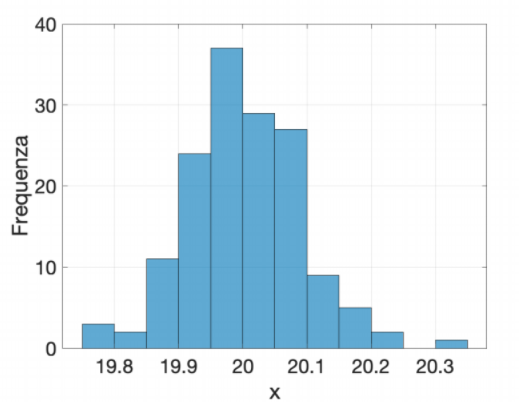
\includegraphics[width=5cm]{isto-a} \caption{}
			\end{subfigure}
			\begin{subfigure}{0.45\linewidth}
				\centering
				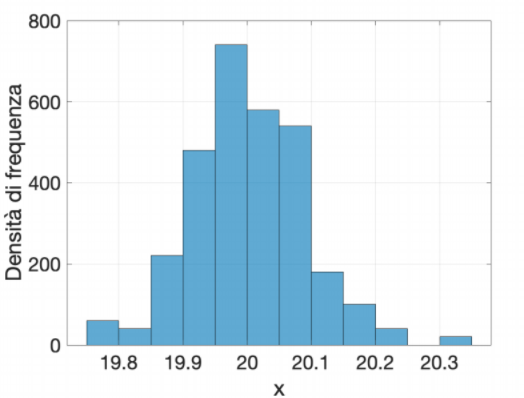
\includegraphics[width=5cm]{isto-b} \caption{}
			\end{subfigure}
			\begin{subfigure}{0.45\linewidth}
				\centering
				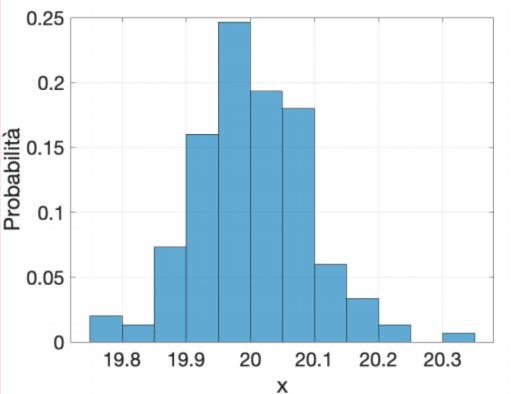
\includegraphics[width=5cm]{isto-c} \caption{}
			\end{subfigure}
			\begin{subfigure}{0.45\linewidth}
				\centering
				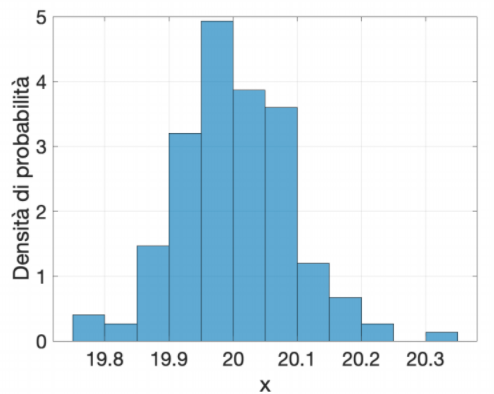
\includegraphics[width=5cm]{isto-d} \caption{}
			\end{subfigure}
			\caption{istogramma di frequenza (a), densità di frequenza (b), probabilità (c) e densità di probabilità (d) delle misurazioni di uno stesso campione. } \label{fig:stat:istogrammi}
		\end{figure}
		
		Il numero di classi (e la loro ampiezza) è in generale arbitraria e può non essere omogeneo; tuttavia è possibile utilizzare le cosiddette \de{formule di \textit{binning}} per stabilire il numero \textit{ideale} di classi $n$ da rappresentare in funzione del numero di campioni $N$:
		\begin{align*}
			\textrm{eq. di Scott:} & \qquad n = 3.5 s_x N^{-1/3} \\
			\textrm{eq. di Sturges:}& \qquad n = \lceil{1 + \log_2(N) \rceil}
		\end{align*}
		In queste relazioni il termine $s_x$ rappresenta la deviazione standard del campione analizzato.
		
		\paragraph{Diagramma cumulato} Un numero alternativo di rappresentare i dati tramite la cumulazione delle classi precedenti, come si può osservare in figura \ref{istocum}. Ogni \textit{canna} rappresenta dunque il numero di osservazioni inferiori al valore rispetto al quale si riferisce.
	
		\figura{5}{1}{isto-cum}{istogramma cumulato della frequenza ottenuto dagli stessi dati degli istogrammi in figura \ref{fig:stat:istogrammi}.}{istocum}
	
	
\section{Stimatori} 
	Uno \de{stimatore} (o \textbf{statistica}) è un operatore che determina un valore numerico associato alle misurazioni; essi possono stimare la \de{tendenza centrale} del campione (che può essere la media, la moda oppure la mediana) o la \de{dispersione} (come intervallo della classe, varianza e deviazione standard.
		
	\subsection{Stimatori di tendenza centrale}	
		\paragraph{Media} Il primo stimatore di tendenza centrale è la \de{media}; essa è definita come $\mu$ se si sta analizzando una popolazione, mentre $\ov x$ se si analizza un campione della popolazione; in particolare esse sono determinate dalle equazioni matematiche:
		\begin{equation}
			\begin{split}
				\mu &  = \sum_{i=1}^n x_i\, f\big(x_i\big) \qquad  \textrm{: popolazione} \\
				\ov x &  = \sum_{i=1}^n \frac{x_i}{n} \qquad \textrm{: campione} 
			\end{split}
		\end{equation}
		In questa espressione $x_i$ rappresenta il valore della variabile aleatoria che si presenta con una probabilità $f(x_i)$ nel caso della popolazione (nel caso del campione di fatto si effettua una \textit{media ponderata}).
		
		\paragraph{Mediana} La \de{mediana} $\med (x)$ di un campione o di una popolazione rappresenta il \textit{valore di mezzo} tra tutte le variabili aleatorie osservate \textbf{(DISCRETE ? )}; essa deve essere definita in maniera distinta in base al numero $n$ di dati analizzati. Una volta ordinati gli elementi la mediana è determinata dall'equazione
		\begin{equation}
			\med (x) = \left\{ \begin{split}
				\frac{x\left(\frac n 2\right) + x\left(\frac{n+1}{2}\right) }{2} \qquad & \textrm{con $n$ pari} \\
				x\left(\frac {n+1} 2\right)  \qquad & \textrm{con $n$ dispari} \\
			\end{split}\right.
		\end{equation}
			
		\paragraph{Moda} La \de{moda} rappresenta di fatto la variabile aleatoria $x$ più frequente all'interno dei dati analizzati
		
	\subsection{Stimatori di dispersione}
		\paragraph{Intervallo} L'\de{intervallo} $\rng (x_i)$ di una variabile aleatoria $x_i$ rappresenta l'ampiezza della classe associata alla stessa, e dunque
		\begin{equation}
			\rng \big(x_i\big) = \max \big(x_i\big) -  \min \big(x_i\big)
		\end{equation}
		
		\paragraph{Varianza e deviazione standard} La \de{varianza}, denominata $\sigma^2$ per una popolazione e $s^2$ per un campione, è calcolata come \textit{media pesata} della differenza tra variabile considerata e media elevata al quadrata, ossia:
		\begin{equation} \label{eq:stat:varianza}
			\begin{split}
				\sigma^2 &  = \frac{\sum_{i=1}^n \big(x_i-\mu\big)^2}{n} \qquad  \textrm{: popolazione} \\
				s^2 &  = \frac{\sum_{i=1}^n \big(x_i - \ov x\big)^2}{n-1} \qquad \textrm{: campione} 
			\end{split}
		\end{equation}
		
		La \de{deviazione standard} ($\sigma$ per la popolazione, $s$ per un campione) è definita a partire dall'equazione \ref{eq:stat:varianza} come la radice quadrata della varianza.
		
	\subsection{Distribuzioni di probabilità}
		Le \de{distribuzioni di probabilità} possono essere descritte tramite due particolari funzioni: la \de{PDF} (\textit{probability density function}, denotata generalmente come $f_{pd}$ e la \de{CDF} (\textit{cumulative density function}), denominata $f_{cd}$, definita come:
		\begin{equation}
			f_{cd} \big(x_i\big) = \int_{-\infty}^{x_i} f_{pd}(\xi)\, d\xi
		\end{equation}
		La funzione $f_{pd}(x_i)$ indica di fatto la probabilità (o la sua densità) della variabile aleatoria $x_i$.
		
		Utilizzando un istogramma cumulato, ossia descritto da una funzione CDF, la probabilità $P$ di riscontrare un valore $x$ in un intervallo $(a,b)$ può essere determinata come
		\[ P\big(a< x < b\big) = f_{cd}(b) - f_{cd}(a) \]
		Il problema di questo tipo di formulazione è che raramente si conosce l'intera popolazione e che spesso la \textit{forma degli istogrammi}, ossia la loro \de{distribuzione}, può essere diversa per diverse variabili.
		
		\vspace{3mm} Definire delle \textbf{distribuzioni di riferimento} in \textbf{termini matematici} consente di calcolare la probabilità di una variabile aleatoria senza conoscere l'intera popolazione; è dunque possibile identificare tale distribuzione di riferimento studiando il comportamento di un campione casuale della stessa. \\ 
		A tale fine sono descritte delle distribuzioni di probabilità sia per variabili discrete (come il lancio di un dado), sia per variabili continue; in questo corso si porrà attenzione solo su quest'ultime in quanto sono quelle utilizzate nelle misurazioni.
	
		\paragraph{Media e varianza} La media $\mu$ e la varianza $\sigma^2$ di una popolazione possono essere determinate mediante l'utilizzo rispettivamente dell'\de{operatore valore atteso} $E(y)$ e l'\de{operatore della varianza} $V(y)$; sono dunque qui riportate le formulazioni di entrambi gli operatori sia per distribuzioni discrete (sommatoria) che continue (integrale):
		\begin{equation}
		\begin{split}
			\mu & := E(y) = \left\{ \begin{split}
				\sum_i y_i \, p\big(y_i\big) \\
				\int_{-\infty}^\infty y\, f(y)\, dy
			\end{split} \right. \\
			\sigma^2 & := V(y) = \left\{ \begin{split}
					\sum_i \big(y_i - \mu\big)^2 \, p\big(y_i\big) \\
					\int_{-\infty}^\infty \big(y -\mu\big)^2\, f(y)\, dy
				\end{split} \right. \\
				&= E\Big( (y-\mu)^2\Big)
		\end{split}
		\end{equation}
		
		In queste equazioni si indica con $p(y_i)$ la probabilità della variabile aleatoria $y_i$, mentre con $f(y)$ la probabilità della variabile $y$ definita dalla PDF associata.
		
		
		\paragraph{Proprietà degli operatori} Proprietà fondamentali dell'operatore valore atteso è che il valore atteso di una costante $c$ coincide con se stesso, mentre la varianza della stessa è sempre nulla:
		\[ E(c) = c  \quad V(c) = 0 \qquad  \forall c \in \mathds R\]
		Si dimostra che il valore atteso è un operatore lineare, ossia date due costante $c_1,c_2$ e due medie ($\mu_1 = E(y_1)$ ottenuta da un primo campione  e $\mu_2 = E(y_2)$ ottenuta da un secondo campione) allora vale che
		\[ E\big(c_1y_1 + c_2 y_2\big) = c_1 E\big(y_1\big) + c_2 E\big(y_2\big) = c_1 \mu_1 + c_2 \mu_2 \]
		Per quanto riguarda la varianza, noto che per un campione $y$ si ha $\sigma^2 = V(y)$, per ogni costante $c\in \mathds R$ allora deve valere che
		\[  V\big(cy\big) = c^2 V\big(y\big) = c^2\sigma^2 \]
		
		Si introduce inoltre la \de{covarianza} di due valori $y_1,y_2$ definita come
		\begin{equation}
			\cov\big(y_1,y_2\big) = E \Big((y_1-\mu_1) (y_2-\mu_2)\Big)
		\end{equation}
		Tramite questa definizione è possibile verificare le seguenti relazioni valore per l'operatore varianza:
		\[V\big(y_1+y_2\big) = V\big(y_1\big) + V\big(y_2\big) + 2 \cov \big(y_1,y_2\big) \qquad V\big(y_1-y_2\big) = V\big(y_1\big) + V\big(y_2\big) - 2 \cov \big(y_1,y_2\big) \]
		
		\textbf{DA FINIRE e CHIEDERE DELLE PRECISAZIONI}
		
	\subsection{Principali distribuzioni continue}
		
		Innanzitutto, come visto in precedenza, è possibile affermare che la funzione CDF è l'integrale progressivo della rispettiva PDF $f_{pd}(x)$; in particolare esiste la funzione CDF \textbf{\textit{lower tail}} $f_{cd,l}(x)$ che integra da $-\infty$, mentre esiste la funzione \textbf{\textit{upper tail}} $f_{cd,u}(x)$ che integra da $+\infty$ e che sono dunque definite come segue:
		\begin{equation}
			f_{cd,l}(x) = \int_{-\infty} ^ x f_{pd}(\xi)\, d\xi \qquad f_{cd,u} = \int_x ^\infty f_{pd} (\xi) \, d\xi = 1-f_{cd,l}(x)
		\end{equation}
		
		In generale la funzione PDF $f_{pd}$ descrive la densità di probabilità di una variabile stocastica; questo significa che per determinare la probabilità che un valore $x$ si trovi nell'intervallo continuo $[a,b]$ è necessario considerare le relazioni
		\begin{align*}
			P\Big(x\in[a,b]\Big) & = \int _a ^b f_{pd}(\xi) \, d\xi \\ 
			&= \int_{-\infty}^b f_{pd}(\xi) \, d\xi - \int_{-\infty}^a f_{pd}(\xi)\, d\xi = f_{cd,l}(b) - f_{cd,l}(a)
		\end{align*}		
		Da queste relazioni risulta evidente che la probabilità di determinare un valore preciso $x=x_0$ è sempre nulla: $P(x=x_0) = 0$.
		
		\paragraph{Comportamento simile} In statistica il termine $\backsim$ serve ad indicare la similarità di comportamento di due espressioni; in particolare date due funzioni di densità di probabilità $x,y$ allora l'espressione $x\backsim$ si può interpretare come \textit{$x$ si comporta come $y$}.
		
		\paragraph{Distribuzione uniforme} E' possibile affermare che una variabile stocastica $y$ si comporta come una \de{distribuzione uniforme} $U(a,b)$, mostrata in figura \ref{fig:stat:uniforme}, nell'intervallo di estremi $a$ e $b$ se la sua PDF segue una formulazione del tipo
		\begin{equation}
			f_{pd}(y) = \begin{cases}
				0 & y < a \textrm{ oppure } y > b \\
				\frac{1}{b-a} \qquad & a\leq y\leq b
			\end{cases}
		\end{equation}
		
		\begin{figure}[bht]
			\centering
			\begin{subfigure}{0.48\linewidth}
				\centering
				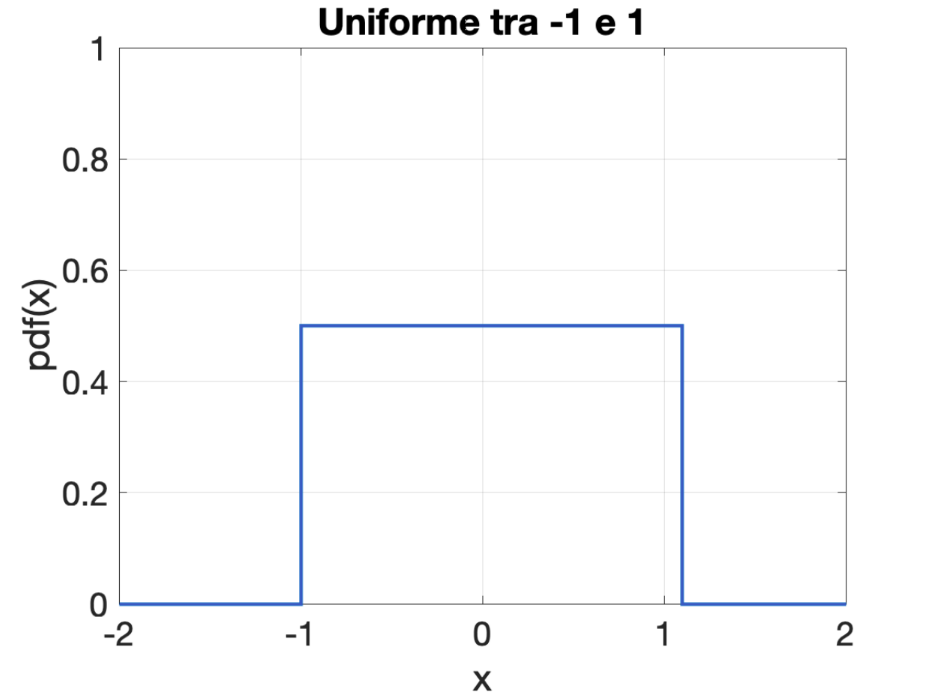
\includegraphics[width=5cm]{uniforme-pdf} \caption{}
			\end{subfigure}
			\begin{subfigure}{0.48\linewidth}
				\centering
				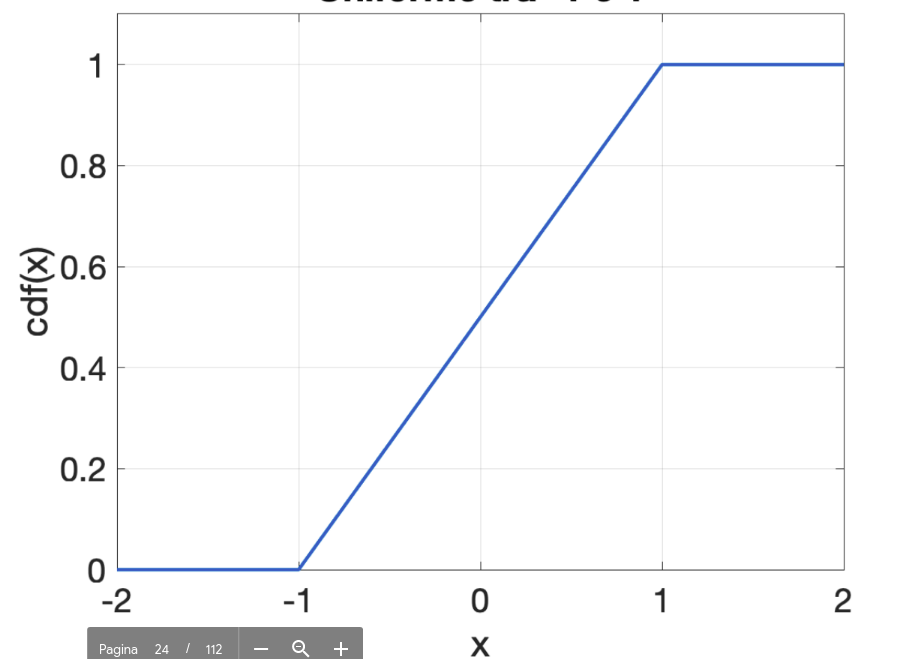
\includegraphics[width=5cm]{uniforme-cdf} \caption{}
			\end{subfigure}
			\caption{funzione PDF (a) e CDF (b) di una distribuzione uniforme $U(-1,1)$.}
			\label{fig:stat:uniforme}
		\end{figure}
		
		\paragraph{Distribuzione normale o gaussiana} Un evento statistico $y$ si comporta come \de{distribuzione normale} (o \de{gaussiana}) $y \backsim N(\mu , \sigma^2)$ di media $\mu$ e varianza $\sigma^2$ (figura \ref{fig:stat:gaussiana}) se al sua PDF segue una relazione del tipo
		\begin{equation}
			f_{pd}(y) = \frac 1 {\sigma \sqrt{2\pi}} e^{-\dfrac 1 2 \left[\dfrac{y-\mu}{\sigma}\right]^2}
		\end{equation}
		
		Una generica distribuzione gaussiana di valore atteso $\mu$ e varianza $\sigma^2$ può essere normalizzata per diventare una distribuzione normale di valore atteso $0$ e varianza unitaria secondo la legge
		\begin{equation}
			\frac{y -\mu}{\sigma} \backsim N(0,1)
		\end{equation}
		Caratteristica della distribuzione gaussiana normalizzata è che la probabilità di ottenere un valore stocastico $x$ nell'intervallo $(-3,3)$ è pari al $99.7\%$.
		
		
		\begin{figure}[bht]
			\centering
			\begin{subfigure}{0.48\linewidth}
				\centering
				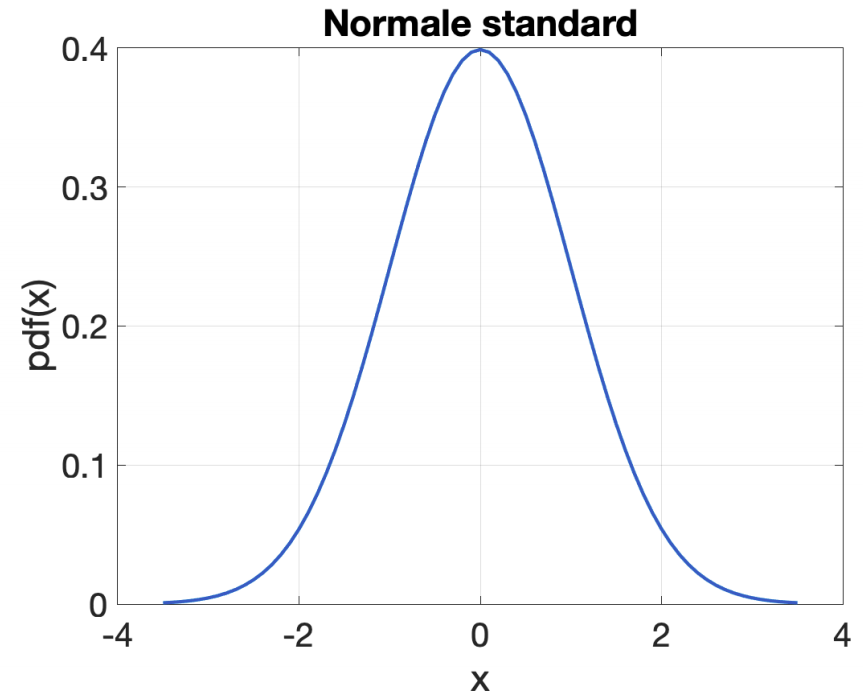
\includegraphics[width=5cm]{gaussiana-pdf} \caption{}
			\end{subfigure}
			\begin{subfigure}{0.48\linewidth}
				\centering
				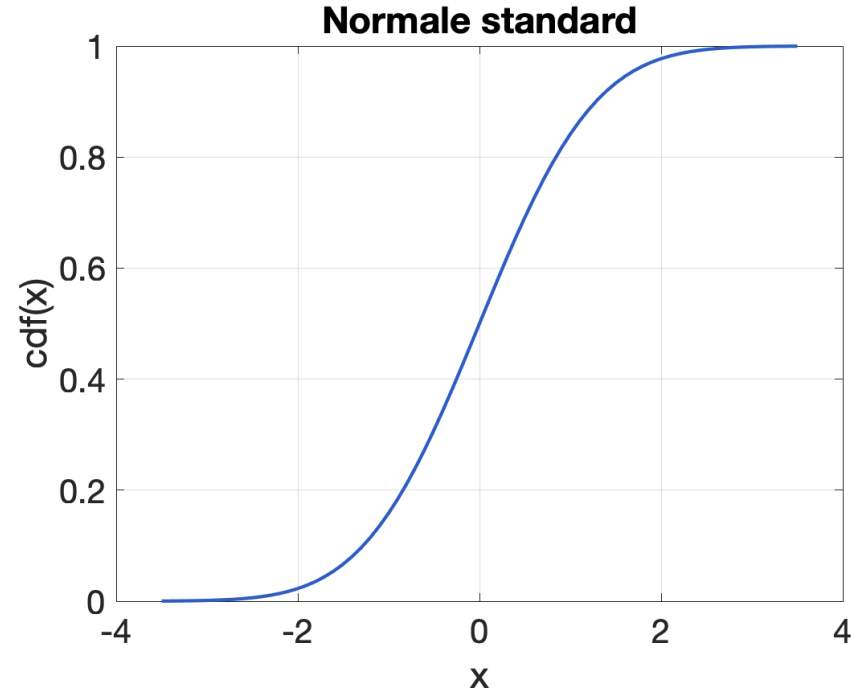
\includegraphics[width=5cm]{gaussiana-cdf} \caption{}
			\end{subfigure}
			\caption{funzione PDF (a) e CDF (b) di una distribuzione gaussiana standard $N(0,1)$.}
			\label{fig:stat:gaussiana}
		\end{figure}
		
		\paragraph{Distribuzione chi-quadro} Un variabile stocastica $y$ è approssimata ad una \de{distribuzione xhi-quadro} $\chi^2_k$ di ordine $k$ (figura \ref{fig:stat:chiquadro}) se può essere scritta come una somma di distribuzioni normali al quadrato:
		\begin{equation}
			y \backsim \chi_k^2 \qquad \Leftrightarrow \qquad y = z_1^2 + z_2^2 + \dots + z_k^2 \quad \textrm{con } z_i\backsim N(0,1)
		\end{equation}
		La funzione PDF $f_{pd}(y)$ può essere calcolato utilizzando la funzione gamma $\Gamma$ di Eulero ed è determinata come
		\begin{equation}
			f_{pd}(y) = \frac 1 {2^{k/2} \, \Gamma \big(k/2\big) } y ^{\frac k 2 - 1} e^{-\frac y 2}
		\end{equation}
		Di questa distribuzione è possibile osservare che il valore atteso $\mu$ coincide con l'ordine della funzione, ossia $\mu = k$; la varianza della stessa risulta essere invece $\sigma^2 = 2k$.
		
		Definendo con $ss$ la somma degli scarti quadratici medi di un campione di media $\ov y$, allora il suo rapporto con lo scarto quadratico medio $\sigma^2$ della relativa popolazione si distribuisce come una chi-quadro secondo la relaizone
		\begin{equation}
			\frac{ss}{\sigma^2} = \frac{\sum_{i=1}^2 \big(y_i-\ov y\big)^2}{\sigma^2} \backsim \chi_{n-1}^2
		\end{equation}
		
		\begin{figure}[bht]
			\centering
			\begin{subfigure}{0.48\linewidth}
				\centering
				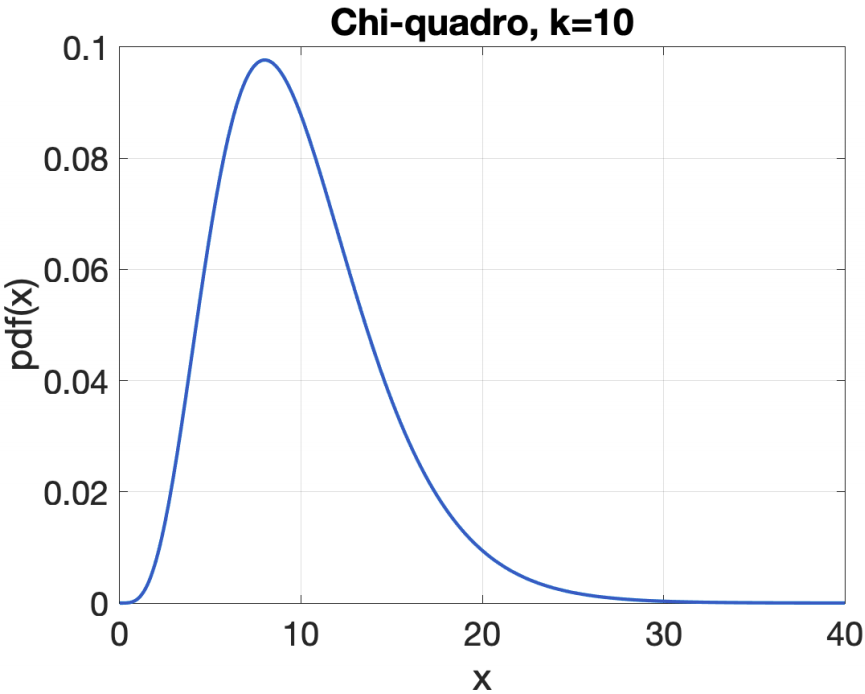
\includegraphics[width=5cm]{chiquadro-pdf} \caption{}
			\end{subfigure}
			\begin{subfigure}{0.48\linewidth}
				\centering
				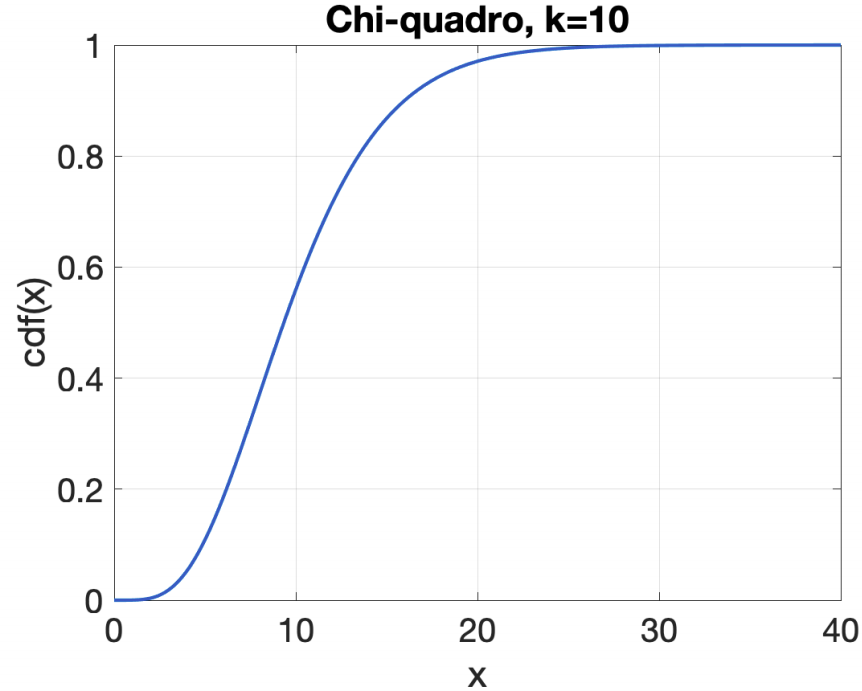
\includegraphics[width=5cm]{chiquadro-cdf} \caption{}
			\end{subfigure}
			\caption{funzione PDF (a) e CDF (b) di una distribuzione chi-quadro $\chi^2_{10}$ di ordine $k=10$.}
			\label{fig:stat:chiquadro}
		\end{figure}
		
		\paragraph{Distribuzione T di Student} Una variabile stocastica $y$ è \de{distribuita} come una \de{T di Student} $y \backsim t_k$ di ordine $k$ se è esprimibile nella forma
		\begin{equation}
			y \backsim t_k \qquad \Leftrightarrow \qquad y = \frac z {\sqrt{x/k}} \quad \textrm{con } z \backsim N (0,1) \ , \ x \backsim \chi_k^2
		\end{equation}
		La relativa PDF può essere espressa come
		\begin{equation}
			f_{pd}(y) = \frac{\Gamma \left(\frac{k-1}{2}\right)}{\sqrt{k\pi} \, \Gamma \left( \frac k 2 \right)} \frac 1 {\left(\frac{y^2}{k} + 1 \right)^{(k+1)/2}}
		\end{equation}
		Questa funzione è caratterizzata dall'avere valore atteso $\mu = 0$ e varianza $\sigma^2 = \frac{k}{k+2}$. E' possibile osservare che per $k\rightarrow \infty$ la distribuzione T di Student tende ad assumere una distribuzione normale (l'approssimazione è valida in generale per $k>50$):
		\[ t_k \quad \xrightarrow{k\rightarrow \infty} \quad N(0,1)\]
		
		\begin{figure}[bht]
			\centering
			\begin{subfigure}{0.48\linewidth}
				\centering
				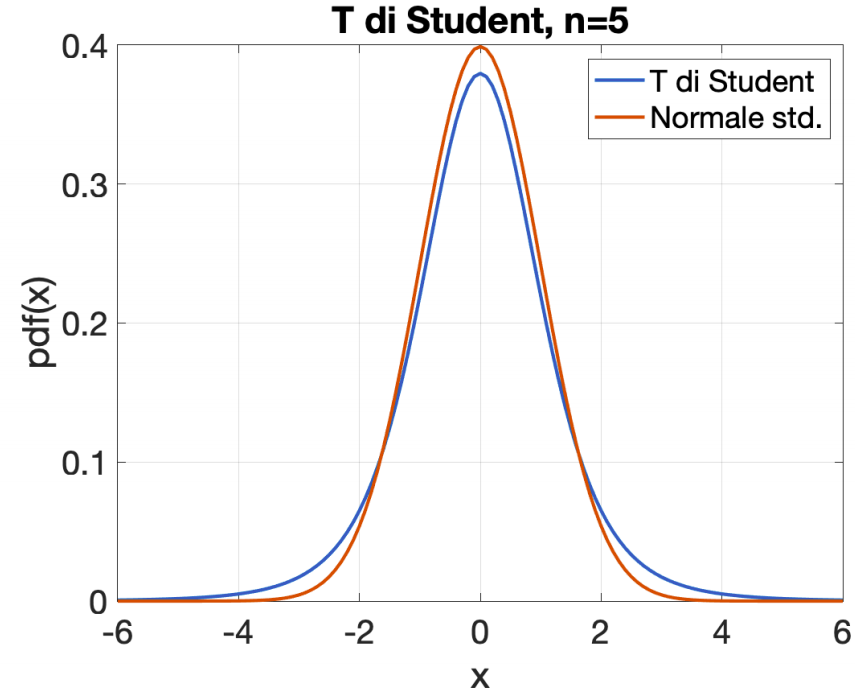
\includegraphics[width=5cm]{student-pdf} \caption{}
			\end{subfigure}
			\begin{subfigure}{0.48\linewidth}
				\centering
				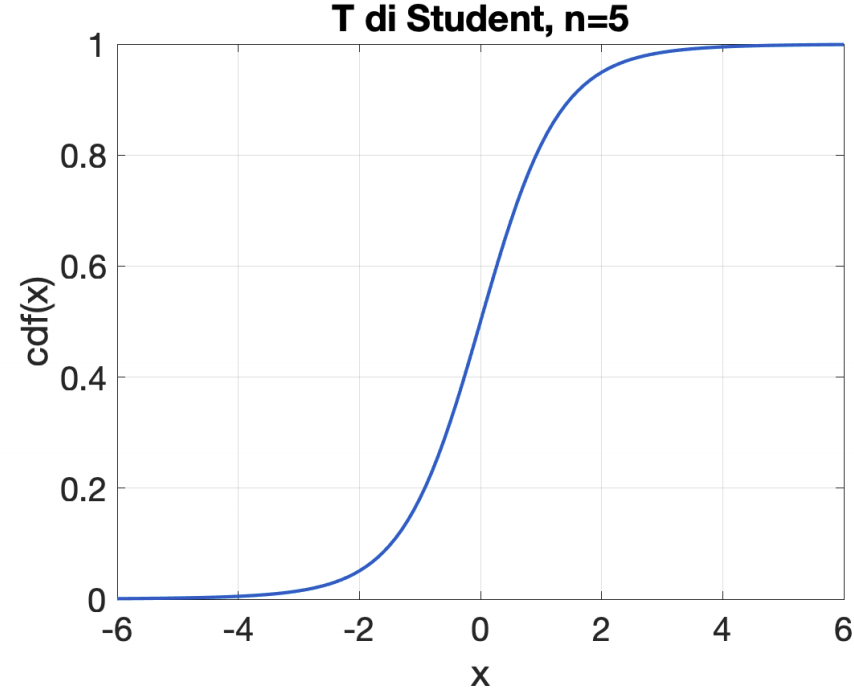
\includegraphics[width=5cm]{student-cdf} \caption{}
			\end{subfigure}
			\caption{funzione PDF (a), in relazione ad una normale, e CDF (b) di una distribuzione T di Student $t_5$ di ordine $k=5$.}
			\label{fig:stat:student}
		\end{figure}
		
		
	\subsection{Distribuzione della media e teorema del limite centrale}
		
		\paragraph{Distribuzione della media} Si consideri $x_i \backsim N(\mu, \sigma^2)$, ossia una variabile aleatoria  con distribuzione normale di valore atteso $\mu$ e varianza $\sigma_2$. E' possibile verificare che la \de{media campionaria} $\ov x$ di un campione assume una distribuzione normale in quanto somma delle stesse:
		\begin{align*}
			E\big(\ov x\big) & = E \left(\frac{x_1 + x_2 + \dots  
			 + x_n}{n}\right) = \frac 1 n \, E\left(x_1 + x_2+\dots +x_n\right) \\ 
		 	& = \frac 1 n \Big[ E(x_1) + E(x_2) + \dots + E(x_n)\Big] = \frac 1 n n E(x) \\
		 	& = \mu 
		\end{align*}
		
		A questo punto è possibile stabilire, tramite l'operatore varianza, la varianza $s_{\ov x}^2$ del campione di variabili $x$ (ognuna delle quali di varianza $s_x^2$) utilizzando le relazioni
		\begin{align*}
			V\big(\ov x\big) & = V \left( \frac{x_1 + x_2 + \dots + x_n}{n} \right) = \left(\frac 1 n\right)^2 \, V\big(x_1+x_2+\dots +x_n\big) \\
			& = \frac 1 {n^2} \Big[ V(x_1) + V(x_2) + \dots + V(x_n) \Big] = \frac n {n^2} V(x) = \frac 1 n V(x) \\
			& = \frac{s_x^2}{n}
		\end{align*}	
		A questo punto è possibile osservare che la distribuzione di una media campionaria di valori di distribuzioni normali è anch'essa una gaussiana di valore atteso $\mu$ ma varianza $\sigma^2/n$ e dunque
		\[ \ov x \backsim N\big(\mu , \sigma^2/n\big) \]	
		
		\subsubsection{Teorema del limite centrale}
		\paragraph{Enunciato} {\itshape Se $x_1,x_2,\dots, x_n$ sono $n$ variabili aleatorie indipendenti ed egualmente distribuite con valore atteso $E(x_i)=\mu$ e varianza $V(x_i) = \sigma^2$ (entrambi valori finiti), e si consideri $y = x_1+x_2+\dots + x_n$, allora
		\[ z_n = \frac{y - n\mu }{\sqrt{n\sigma^2}} \]
		è distribuita approssimativamente come una gaussiana $N(0,1)$ nel senso che, se $F_n(z)$ è la densità di probabilità di $z_n$ e $\Phi(z)$ è la PDF di una variabile casusale di tipo $N(0,1)$, allora
		\[\lim_{n\rightarrow \infty} \frac{F_n(z)}{\phi(z)} = 1\] }
		
		\paragraph{Osservazioni} Da questo teorema deriva il fatto che la distribuzione gaussiana è detta normale in quanto occupa un posto centrale per il limite a cui tendono le distribuzioni delle somme. Questo è un teorema molto robusto rispetto alle ipotesi: ogni  misurazione dipende da numeri fattori casuali (dovuti al misurando, ai trasduttori, ai rumori ambientali e dell'operatore..) che determina con elevata probabilità che la componente casuale dei valori sia distribuita in maniera normale.
		
\section{Statistica inferenziale}
	La \de{statistica inferenziale} è il procedimento per cui si inducono le caratteristiche di una popolazione dall'\textbf{osservazione di un campione estratto a caso} della stessa. 
	
	Una parte fondamentale della statistica inferenziale sono i \de{test statistici}, ossia dei particolari tesi in cui ci si domanda se un dato campione sia o meno compatibile con la rispettiva popolazione di riferimento (valutandone il valore atteso, la varianza e la distribuzione). \\
	In particolare un test statistico serve a decidere quale di due \textbf{ipotesi opposte} ha più probabilità di essere errata; si definiscono dunque l'\de{ipotesi nulla} $H_0$ quella debole (che tipicamente corrisponde ad un'osservazione non significativa) e l'\de{ipotesi alternativa} $H_1$ come la scelta forte, diversa dal valore atteso. In linea di principio dato un campione di media campionaria $\ov x$ e valore atteso della popolazione $\mu_0$ le due ipotesi sono caratterizzate dall'espressione
	\[ H_0:\ \ov x \simeq  \mu_0 \qquad H_1:\ \ov x \neq \mu_0 \]
	
	\begin{esempio}{: ipotesi in un impianto industriale} \label{es:stat:impianto}
		Considerando di vole effettuare un test statistico su un impianto industriale (per esempio verificare che i diametri dei tubi siano coerenti rispetto al valore richiesto) allora:
		\begin{itemize}
			\item l'ipotesi nulla $H_0$, quella debole, è associata al corretto funzionamento dell'impianto in quanto la distribuzione dei campioni analizzati è in linea con la distribuzione teorica della fabbrica;
			\item l'ipotesi alternativa $H_1$, quella forte, è associata ad uno scorretto funzionamento dell'impianto che produce tubi con diametri statisticamente incompatibili con il valore nominale.
		\end{itemize}
	\end{esempio}
	
	Le ipotesi si raggruppano tipicamente nella cosiddetta \de{matrice di confusione} che correla la verità dell'ipotesi nulla $H_0$ con la decisione presa di accettarla o rifiutarla:
	\begin{SCtable}[0.5][h!]
		
		\begin{tabular}{ c | c c}
			$H_0$ &  vera & falsa \\ \hline \hline 
			accettata & ok & {$\beta$: errore di tipo II  } \\
			rifiutata & $\alpha$: errore di tipo I  & ok
		\end{tabular}
		
		\caption{matrice di confusione.}
	\end{SCtable}
	
	Si può osservare che accettando l'ipotesi nulla quando essa è verifica (e analogamente rifiutarla quando essa è falsa) comporta una scelta corretta del comportamento da seguire
	
	L'\de{errore di tipo I} può essere considerato come un \textbf{falso allarme} e si verifica quando si rifiuta un'ipotesi nulla vera; questo tipo di errore è valutato dal parametro $\alpha$.	Accettando invece l'ipotesi falsa si ha un \de{errore di tipo II}, ossia un \textbf{mancato allarme}, ed è valutato dalla probabilità $\beta$; il termine $1-\beta$ rappresenta dunque la \de{potenza} del test statistico. I valori $\alpha$ e $\beta$ non sono necessariamente correlati.
	
	\begin{esempio}{: matrice di confusione in un impianto industriale}
		Facendo riferimento all'esempio \ref{es:stat:impianto}, è possibile associare la matrice di confusione ai seguenti stati di funzionamento con l'obiettivo di fermare l'impianto nel caso in cui esso produca pezzi non congruenti all'obiettivo.
		
		Nel caso in cui l'ipotesi nulla $H_0$ sia verificata allora l'impianto sta producendo correttamente i pezzi:
		\begin{itemize}
			\item accettando l'ipotesi l'impianto continuerà a produrre ed è una scelta corretta, in quanto non ci sono problemi di funzionamento del sistema;
			\item rifiutando questa ipotesi allora si considera che il sistema stia producendo pezzi difettosi quando la realtà è diversa: si ha dunque un falso allarme in quanto l'impianto si fermerebbe nonostante dovrebbe continuare a produrre.
		\end{itemize}
	
		Nel caso in cui l'ipotesi nulla $H_0$ sia falsa allora l'impianto sta producendo pezzi non conformi all'obiettivo:
		\begin{itemize}
			\item rifiutando l'ipotesi l'impianto si ferma  in quanto è riuscito ad individuare correttamente il suo malfunzionamento;
			\item accettando invece l'ipotesi nulla allora l'impianto, nonostante stia sbagliando, pensa di produrre i pezzi in maniera corretta ed è per questo che si parla di mancato allarme: l'impianto non rileva uno stato di funzionamento erroneo.
		\end{itemize}
	\end{esempio}

	\subsection{Analisi di un campione}  \label{sec:stat:teststudent}
		\paragraph{Test di Student} Considerando un campione di $n$ valori aleatori $x_i$ è possibile standardizzare la media campionaria $\ov x$ sottraendo alla stessa il valore atteso $\mu_0$ del test e dividendo il tutto per la deviazione standard del campione (divisione $s/\sqrt n$) ottenendo il risultato
		\[ t_0 = \frac{\big|\ov x- \mu_0\big|}{s/\sqrt n} \backsim t_n \]
		Si osserva dunque che il risultato normalizzato è distribuito come una t di student con parametro $n$ pari al numero di campioni. Il risultato $t_0$ è detto dunque \de{statistica di test}.
		
		Intuitivamente la statistica $t_0$ è tanto più grande quanto più la media campionaria è distante dal valore atteso relativamente alla sua varianza. Tanto più è piccola la probabilità di riscontrare un valore maggiore di $t_0$ sulla distribuzione T di Student, tanto più possiamo dedirre che il campione con media $\ov x$ e varianza $s^2$ \textbf{non proviene} da una popolazione con valore atteso $\mu_0$. La probabilità di riscontrare un valore maggiore di $t_0$ è dunque detto \de{\textit{p-}value} e rappresenta la probabilità di errore di tipo I $\alpha$.
		
		\begin{esempio}{: \textit{p-}value}
			Considerando un campione di $n=5$ elementi con media campionaria $\ov x$ e varianza $s^2$ tali da generare una statistica di test $t_0=2$:
			\[ t_0 = \frac{|\ov x - \mu_0|}{s/\sqrt 5} = 2 \]
			Determinata la funzione CDF lower tail $f_{cd,l}(t)$ associata alla distribuzione T di Student di parametro 5, allora è possibile determinare il $\pval$ di questa statistica come
			\[ \pval = 2\Big[1- \, f_{cd,l}(t_0) \Big] = 2\, f_{cd,u}(t_0) = 0.046 \]
			Questo significa che la probabilità di errore di affermare che la differenza tra $\ov x$ e $\mu_0$ è significativa è pari al $4.6\%$.
			
			\vspace{3mm}
			Si osserva che nell'espressione del $\pval$ si ha la moltiplicazione per un fattore 2 dovuta al fatto che la distribuzione T di Student è simmetrica ed è necessario considerare anche il rispettivo valore negativo di $t_0$.
		\end{esempio}
		
		Ipotizzando di conoscere la varianza $\sigma^2$ della popolazione della quale si estrae il campione, allora la statistica di test risutla distribuita come una normale standard e assume la forma
		\[ z_0 = \frac{|\ov x - \mu_0|}{\sigma/\sqrt n} \backsim N(0,1) \]
		In generale più $n$ è grande più la distribuzione $t_k$ T di Student di ordine $k$ assomiglia ad una normale standard $N(0,1)$; in generale per un numero di campioni $n>50$ è possibile effettuare l'approssimazione di $t_0$ alla rispettiva distribuzione normale: $t_0\approx z_0$.
		
		
	\subsection{Analisi di normalità}
		L'\de{analisi di normalità} serve per verificare se un campione è più o meno compatibile con una distribuzione normale ed è basata su due tipi di analisi:
		\begin{itemize}
			\item \textbf{analisi dei quantili} del campione e relativo confronto con i quantili di una distribuzione normale; questo è un approccio grafico e dunque soggettivo;
			\item \textbf{analisi} basata su \textbf{test statistici} dove si considera come ipotesi nulla $H_0$ che la distribuzione analizzata sia normale; questo è un approccio oggettivo.
		\end{itemize}
		
		\subsubsection{Analisi dei quantili}
		Il \de{quantile} può essere considerato come la funzione inversa della cumulata di una distribuzione.
		
		
		
		\subsubsection{Test del chi-quadro} 
		Un test statistico per determinare la normalità (o meno) di una distribuzione campionaria può essere effettuato tramite il cosiddetto \de{test del chi-quadro}. 
		
		Essendo questo un test statistico si considera come \textbf{ipotesi nulla} $H_0$ quella che afferma che il campione è distribuito normalmente, mentre l'\textbf{ipotesi alternativa} $H_1$ è quella riferita alla non normalità di distribuzione del campione.
		
		Per effettuare il test è necessario dividere gli $n$ campioni da analizzare in $k$ classi di 4-5 valori l'una. Definendo $O_i$ il numero di osservazioni nell'$i-$esima classe, ad ognuna di esse sarà associato un valore atteso $E_i$ rispetto ad una distribuzione normale che può essere determinata tramite la sua CDF come
		\[ E_i = f_{cd,l}\big(\textrm{max}_k \big) - f_{cd,l}\big(\textrm{min}_k\big)\]
		A questo punto è possibile determinare la \de{statistica di test} $X_0^2$ per il test statistico in questione come
		\[ X_0^2 = \sum_{i=1}^k \frac{\big(O_i - E_i\big)^2}{E_i} \backsim 	\chi^2_{k-p-1}  \]
		
		La statistica di test è una somma di quadrati di variabili casuali ed approssima dunque la distribuzione chi-quadro come indicata; questa approssimazione è tanto più fedele quanto maggiore è il numero di campioni analizzati. Il parametro della distribuzione $\chi^2$ è il numero di elementi indipendenti nella somma che coincide al valore $k-1-p$, dove $k$ è il numero di classi individuate e $p$ è il numero di parametri della distribuzione di riferimento (2 per la distribuzione normale: $\mu$ e $\sigma^2$).
		
		Come nel caso del test T di Student, il $\pval$ del test statistico in questione è determinato dalla probabilità di trovare il valore $X_0^2$ nella distribuzione $\chi^2$; non essendo questo test simmetrico il $\pval$ è determinato tramite la CDL della distribuzione chi-quadro come
		\[\pval = \min \Big\{f_{cd,l}\big(X_0^2\big), f_{cd,u}\big(X_0^2\big)\Big\}\]
		Il $\pval$ rappresenta dunque l'errore nel rigettare l'ipotesi nulla, ossia l'errore che si commetterebbe a considerare la distribuzione di partenza come non normale.
		
		\begin{nota}
			Il test del chi-quadro può essere effettuato non solo per verificare la normalità di una distribuzione, ma per effettuare un confronto tra qualsiasi distribuzione: per fare questo è sufficiente sostituire al criterio di normalità $E_i$ la relazione del valore atteso della distribuzione di riferimento.
		\end{nota}
		
		\subsubsection{Test di contingenza}
		In certi casi $n$ elementi di una popolazione possono essere \textbf{classificati} secondo \textbf{due criteri differenti}: in tal caso è interessante sapere se i due criteri di classificazione siano \textbf{statisticamente indipendenti} o meno.
		
		A questo punto i dati osservati $O_{ij}$ possono essere raggruppati nella cosiddetta \de{tabella di contingenza} che riporta nelle righe il numero di osservazioni che ricadono nel primo criterio, nelle colonne quelle del secondo criterio.
		
		Per effettuare un test di contingenza si consideri il caso di voler sapere se 3 piani di assicurazioni distinti sono preferiti da impiegati salariati o a cottimo basandoci sulla seguente tabella di contingenza:
		\begin{center}
		\begin{tabular}{ c || p{1.5cm} p{1.5cm} p{1.5cm} | c}
			& \multicolumn{3}{c |}{piano assicurativo} & \\
			impiego & \centering piano 1 & \centering piano 2 & \centering piano 3 & totale \\ \hline \hline
			salariato & \centering 160 & \centering 140 & \centering 40 & 340 \\
			a cottimo & \centering 40 & \centering 60 & \centering 60 & 160 \\ \hline 
			totale & \centering 200 & \centering 200 & \centering 100 & 500
		\end{tabular}
		\end{center}
	
		Della tabella è necessario determinare i totali cumulativi sia per riga che per colonna; dividendo questi valori per le osservazioni totali si determinano i \de{totali marginali} $\hat u_i$ (della riga $i-$esima) e $\hat v_j$ (per la colonna $j-$esima); in particolare definendo con $r$ il numero di righe e $c$ il numero di colonne, allora i totali marginali in maniera esplicita sono determinati come
		\[ \hat u_i = \frac 1 n \sum_{j=1}^c O_{ij} \qquad \hat v_j = \frac 1 n \sum_{i=1}^r O_{ij} \]
		Rispetto alla tabella di contingenza in esempio è possibile affermare che i totali marginali per riga valgono $\hat u_1 = 340/500 = 0.68, \hat u_2 = 160/500 = 0.32$, mentre per le colonne $\hat v_1 = 200/500 = 0.4, \hat v_2 = 0.4, \hat v_3 = 0.2$.
		
		Questi totali marginali sono due criteri indipendenti e rappresentano i valori attesi di ciascun criterio: possono dunque essere utilizzati per calcolare i valori attesi $E_{ij}$ di ogni combinazione di criteri:
		\[ E_{ij} = n \hat u_i \hat v_j = \frac 1 n \sum_{j=1}^c O_{ij} \, \sum_{i=1}^r O_{ij} \]
		
		A questo punto è possibile effettuare un \textbf{test chi-quadro} considerando come espressione del valore atteso quella appena descritta, e in particolare si determina la \de{statistica di test} $X_0$ da confrontare con la distribuzione $\chi^2$:
		\[X_0^2 = \sum_{j=1}^c \sum_{i=1}^r \frac{\big(O_{ij} - E_{ij} \big)^2}{E_{ijx}}\]
		
		Il $\pval$ associata alla distribuzione rappresenta l'errore statistico nel considerare i due eventi come dipendenti.
		
	\subsection{Anomalie}
		Un'\de{anomalia} (\textit{outlier}) è un'osservazione non compatibile con la distribuzione del resto del campione; essa più risultare da un errore nella conduzione della misura o nella trascrizione/registrazione del valore misurato stesso.
		
		Questo è un \textbf{evento raro} associato ad una distribuzione differente da quella tipica del processo di misura correttamente eseguito; in generale ci si attende non più di un'anomalia per campione (altrimenti si potrebbe pensare che i valori siano dovuti ad una somma di distribuzioni) e devono dunque essere eliminate per ridurre la varianza della distribuzione rispetto al valore atteso. Le anomalie hanno chiaramente effetti più forti su campioni piccoli.
		
		Per la rimozione delle anomalie è possibile utilizzare il \de{criterio di Chauvenet} o il \de{test di Grubb}, con l'accortezza di non applicare ciascun criterio più di una volta.
		
		\paragraph{Criterio di Chauvenet} Data una serie di $n$ osservazioni $x_i$ che generano una media campionaria $\ov x$ e deviazione standard $s_x$, allora è possibile calcolare lo scarto massimo assoluto $s_0$ come
		\[ s_0 = \max_{i=1,\dots, n} \left(\frac{|x_i - \ov x|}{s_x}\right)  \] 
		
		A questo punti si calcola la probabilità $P_s$ di avere un valore maggiore di $s_0$ sulla normale standard usando le funzioni PDF e CDF della stessa, e dunque:
		\[P_s =P\big(x>s_0\big) = \int_{s_0}^{+\infty} f_{pd}(\xi)\, d\xi = 1 - f_{cd,l}\big(s_0\big) = f_{cd,u}\big(s_0\big)  \]
		
		Su $n$ osservazioni, il numero di elementi attesi con scarto maggiore di $s_0$ è pari ad $n\, P_s$; se tale valore è inferiore a $n\, P_s < 0.5$ allora si elimina il dato con lo scarto maggiore assoluto.
		\begin{nota}
			La procedura non può essere ripetuta più di una volta in quanto porta ad un'alterazione della distribuzione.
		\end{nota}
	
		\paragraph{Test di Grubb} Il \de{test di Grubb} è un metodo statistico per eliminare le anomalie; analogamente date $n$ osservazioni $x_i$ si determina lo scarto massimo assoluto $s_0$ dipendente dalla media campionaria $\ov x$ e la relativa deviazione standard $s_x$. A questo punto si deve verificare se
		\[ s_0 > \frac{ n - 1}{n} \sqrt{\frac{t^2_{\alpha/(2n), n-2}}{n-2+t^2_{\alpha/(2n), n-2}}} \]
		dove $t_{\alpha,k}$ è il quantile $\alpha$ della distribuzione T di Student con parametro $k$.
		
		Se la disuguaglianza risulta essere verificata allora si elimina l'osservazione associata allo scarto massimo $s_0$.
		
\section{Analisi di regressione}		
	L'\de{analisi di regressione} è una serie di strumenti matematici che servono ad identificare i parametri di una legge, ossia un \textbf{modello matematico}, che meglio adattano la stessa a delle osservazioni.
	
	In particolare il \de{modello} è una funzione $f$ che determina la \de{risposta} $y$ in relazione al \de{predittore} $x$ secondo l'espressione $y = f(x)$.
	
	\figura{5}{1}{regressione}{dati campionari (puntini) e relativa funzione di regressione (linea rossa continua).}{esregr}
	
	Considerando l'esempio in figura \ref{esregr}, è possibile osservare che i campioni sembrano disporsi secondo una legge quadratica, seguendo dunque un modello $f(x)$ del tipo:
	\[ y = ax^2+bx+c \]
	Effettuare l'analisi di regressione significa dunque determinare i coefficienti $a,b,c$ che meglio adattano il modello ai dati campionari raccolti.
	
	Il modello di partenza del quale fare la regressione può essere sia semplice (come una retta), sia molto complicato (funzioni non lineari implicite), sia monodimensionale che multidimensionale; il \textbf{numero di dimensioni} $n$ di un modello è il numero di predittori $x_1, \dots, x_n$ utilizzati per effettuare la regressione stessa.
	
	Il \de{modello} può essere sia \de{lineare} che \de{non lineare}, e la catalogazione deve essere effettuata osservando i coefficienti, come nell'esempio seguente:
	\[ \textrm{lineare: } y = c_0 +c_1x_1^2+c_2x_1^2+c_3x_2+c_4x_1x_2 \qquad \textrm{non lineare: } y = \frac{c_1x_1 \cos\big(c_2x_2\big)}{c_3x_3}\]
		
	\paragraph{Regressione ai minimi quadrati} In generale per effettuare questo tipo di analisi, ossia determinare i coefficienti che meglio adattano il modello ai campioni, si utilizza la \de{regressione ai minimi quadrati} che adotta come \de{indice di prestazione} $\Phi$ lo scarto quadratico medio sui punti campionati $\big\langle x_1, \dots, x_N\big\rangle$:
	\begin{equation}
		\Phi\big(c_1, \dots, c_n\big) = \sum_{i=1}^N \epsilon_i^2 \qquad \textrm{con} \quad \epsilon_i^2 = y_i- f\big(c_1, \dots, c_n, x_i\big)
	\end{equation}
	La soluzione del problema è dunque la minimizzazione dell'indice di prestazione $\Phi$.
	
	\begin{esempio}{: regressione lineare}
		Per effettuare una \textbf{regressione lineare}, ossia basata sul modello $y = ax + b$, è necessario considerare che la distanza tra modello e campione è data dall'espressione $\epsilon_i = y_i -\big(ax_i+b\big)$, e dunque il problema per essere risolto richiede la minimizzazione dell'indice di prestazione $\Phi$ dipendente solamente dai parametri $a$ e $b$, e dunque
		\[ \min_{a,b} \,\Phi(a,b) = \min_{a,b} \sum_{i=1}^N \Big[y_i - \big(ax_i+b\big)\Big]^2 \]
		Il minimo dell'espressione, che in questo caso è unico, si può trovare imponendo le derivate parziali di $\Phi$ nulle in funzione della posizione dei coefficienti $a,b$, ossia 
		\[ \frac \partial {\partial a} \Phi (a,b) = 0 \qquad  \frac \partial {\partial b} \Phi (a,b) = 0\]
		
		Svolgendo opportunamente i calcoli si dimostra che i valori ottimali dei coefficienti $a$ e $b$ valgono
		\[ a_\textrm{opt} = \frac{C_{xy}}{C_{xx}} \quad b_\textrm{opt} = \ov y - a\ov x \qquad \leftarrow  C_{xx} = \sum_{i=1}^N\big(x_i-\ov x\big)^2 \quad C_{xy} = \sum_{i=1}^N \big(x_i-\ov x\big)\big(y_i-\ov y\big) \]
		
		E' possibile inoltre determinare le varianze degli elementi fondamentali del modello che risultano valere
		\[ \sigma_y^2 = \frac{\sum_{i=1}^N \big[y_i-ax_i+b\big]^2}{N-2} \qquad \sigma_a^2 = \frac{\sigma_y^2}{C_{xx}} \qquad \sigma_b^2 = \sigma_y^2 \frac{\sum_{i=1}^N x_i^2}{N\, C_{xx}} \]
		
	\end{esempio}

	\subsection{Analisi di regressione di modelli lineari}
		Ogni modello di regressione di tipo lineare (nei coefficienti) può essere analizzato utilizzando una notazione matriciale; in particolare facendo riferimento ad un modello quadratico $ax^2 + bx + c$ (ma è possibile intuire che vale in generale per qualsiasi modello a coefficienti lineari) è possibile, date $N$ misurazioni $x_i$ e relativi risultati $y_i$, scrivere l'uscita vettoriale $\vett y$ come prodotto tra una matrice $\mathcal A\in \mathds{ R^{N\times n}}$ e il vettore dei coefficienti $\vett k$:
		\[ \begin{bmatrix}
			x_1^2 & x_1 & 1 \\
			x_2^2 & x_2 & 1 \\
			\vdots && \vdots \\
			x_N^2 & x_N & 1 
		\end{bmatrix} \begin{pmatrix}
			a \\ b \\ c
		\end{pmatrix} = \begin{pmatrix}
			y_1 \\ y_2 \\ \vdots \\ y_3 
		\end{pmatrix} \qquad \leftrightarrow \qquad \mathcal A \vett k = \vett y \]
		Per determinare il vettore dei coefficienti in maniera algebrica è dunque necessario utilizzare degli \textit{stratagemmi} matematici per rendere la matrice $\mathcal A$ quadrata e dunque invertibile, arrivando ai seguenti risultati:
		\begin{equation}
		\begin{split}
			\mathcal A^t \, \mathcal A \vett k & = \mathcal A^t \vett y \\
			\vett k & = \big(\mathcal A^t\mathcal A\big)^{-1} \mathcal A^t \vett y
		\end{split}
		\end{equation}
		
		Si osserva in generale che per effettuare un'analisi di regressione è necessario avere un numero di campioni che è superiore al numero dei coefficienti da determinare del modello.
		
	\subsection{Intervalli di predizione e confidenza} \label{sec:stat:regrpred}
		L'\de{intervallo di predizione} rappresenta la \textit{fascia} di entro la quale una futura osservazione possa ricadere entro una determinata probabilità, per esempio il $95\%$; in generale questo tipo di intervallo presenta un'ampiezza costante rispetto al modello determinato dalla regressione.
		
		L'\de{intervallo di confidenza} rappresenta invece l'intervallo in cui il modello atteso ha una probabilità di ricadere, ossia con quanta probabilità si ha la garanzia che il modello ottenuto dalla regressione sia fedele ai dati analizzati; questo tipo di intervallo non è in generale a sezione costante ma è particolarmente stretto nel \textit{centro} dei campioni analizzati, mentre tende ad \textit{allargarsi} nell'allontanarsi dal valor medio campionario.
		
		\figura{7}{1.2}{intervallipred}{regressione di un modello nominale (noto a priori) con relativi intervallo di predizione e confidenza (entrambi al $95\%$) rispetto ai campioni mostrati.}{intervallipred}
		
		A livello grafico, in linea generale, l'intervallo di predizione è più \textit{esterno} all'intervallo di confidenza, come si può osservare in figura \ref{intervallipred}.
		
	\subsection{Sovraadattamento e sottoadattamento}
		In generale una domanda lecita da porsi è quella di sapere se il campione è stato adattato \textit{bene} o meno dalla regressione: se il modello è appropriato ai dati, allora i residui\footnote{con \textit{residuo} si intende la distanza (con segno) tra il valore misurato $y_i$ del campione e quello che ci si aspetta dal modello $f(x_i)$.} sono casuali, privi di pattern e sono distribuiti normalmente (per via del teorema del limite centrale), e dunque è possibile confermare il risultato effettuando un testo di normalità come il chi-quadro. Un esempio di tale distribuzione è quella in figura \ref{fig:stat:sottoadattamento}.b.
		
		Si parla di \de{sottoadattamento} (\textit{underfitting}) quando è possibile osservare dei pattern nei residui e questo è dovuto alla \textit{poca curvatura} del modello utilizzato per la regressione dei dati, come si può osservare in figura \ref{fig:stat:sottoadattamento}.c.
		
		\begin{figure}[bht]
			\centering
			\begin{subfigure}{0.32\linewidth}
				\centering
				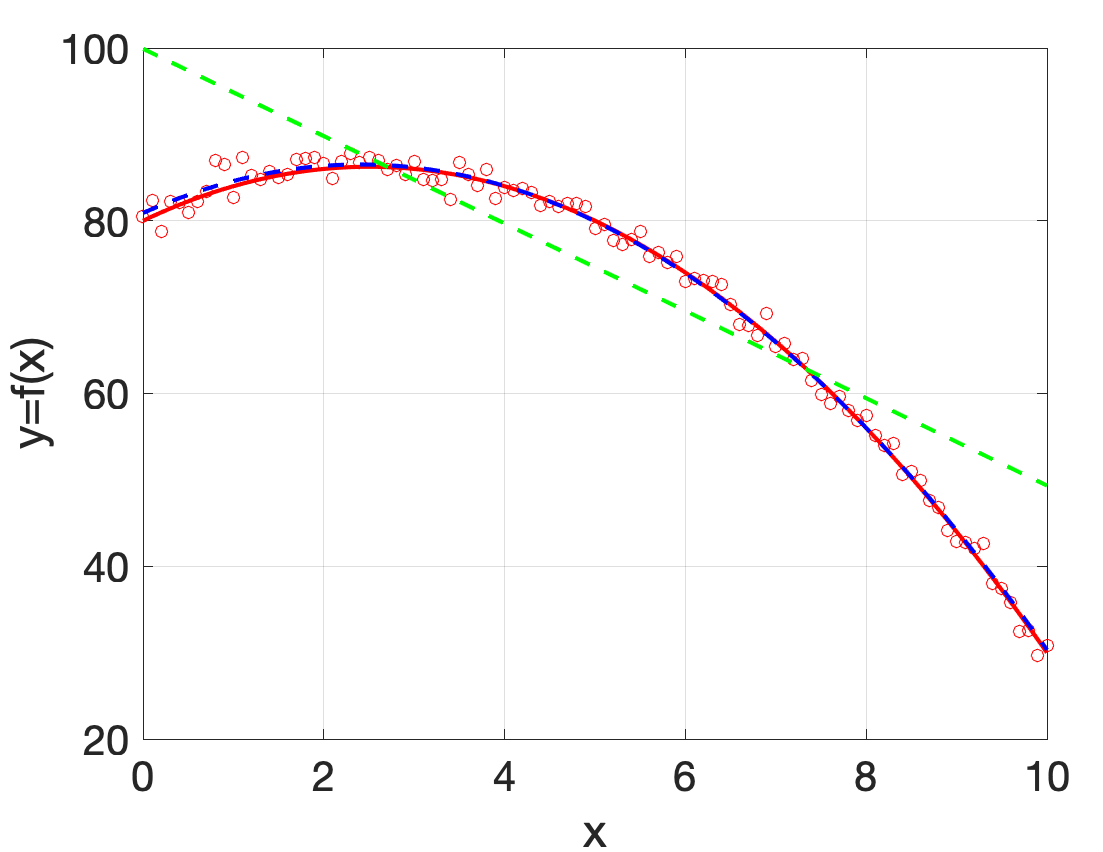
\includegraphics[width=0.9\linewidth]{sotto-a} \caption{}
			\end{subfigure}
			\begin{subfigure}{0.32\linewidth}
				\centering
				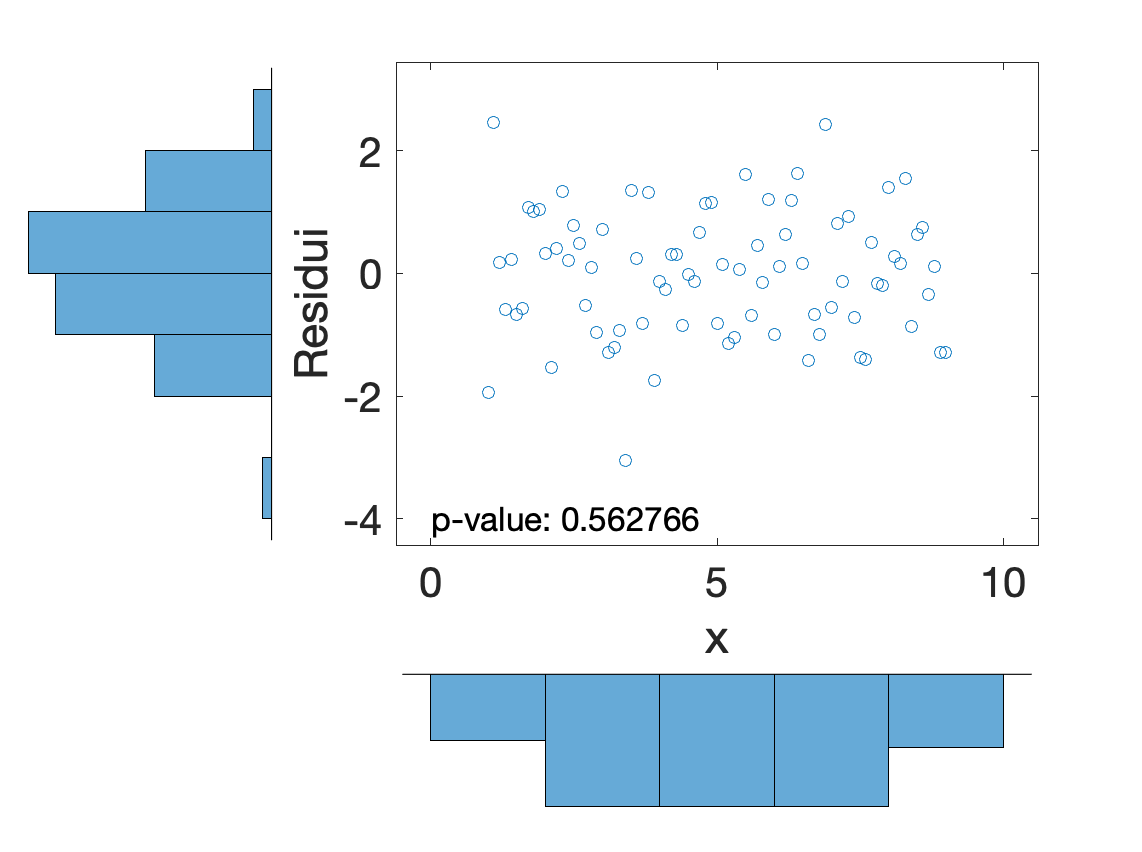
\includegraphics[width=0.9\linewidth]{sotto-b} \caption{}
			\end{subfigure}
			\begin{subfigure}{0.32\linewidth}
				\centering
				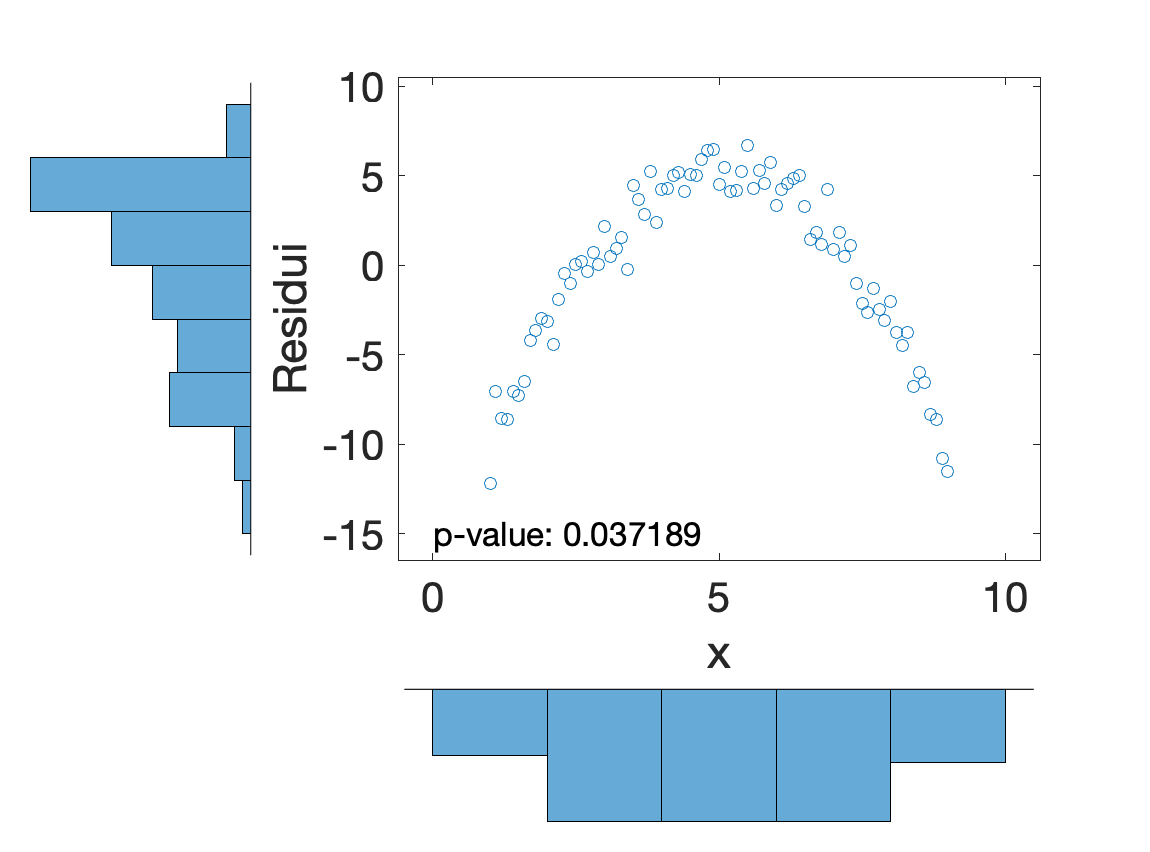
\includegraphics[width=0.9\linewidth]{sotto-c} \caption{}
			\end{subfigure}
			\caption{regressione lineare (in verde) e quadratica (in blu) di campioni distribuiti quadraticamente (curva nominale rossa) in figura $a$; in figura $b$ e $c$ sono mostrati rispettivamente i residui tra campioni e modello nel caso quadratico e lineare.}
			\label{fig:stat:sottoadattamento}
		\end{figure}
	
		Al contrario si parla di \de{sovraadattamento} (\textit{overfitting}) quando il modello utilizzato per effettuare la regressione è di ordine eccessivo al voluto; questo può essere notato considerando che al di fuori dell'\textit{intervallo di addestramento} (rappresentato dalle linee verticali tratteggiate in figura \ref{fig:stat:sovraadattamento}) il modello tende a divergere molto dai valori campionari esterni, e inoltre all'interno di questo range la funzione \textit{oscilla} per inseguire meglio i dati campionari.
		
		\begin{figure}[bht]
			\centering
			\begin{subfigure}{0.49\linewidth}
				\centering
				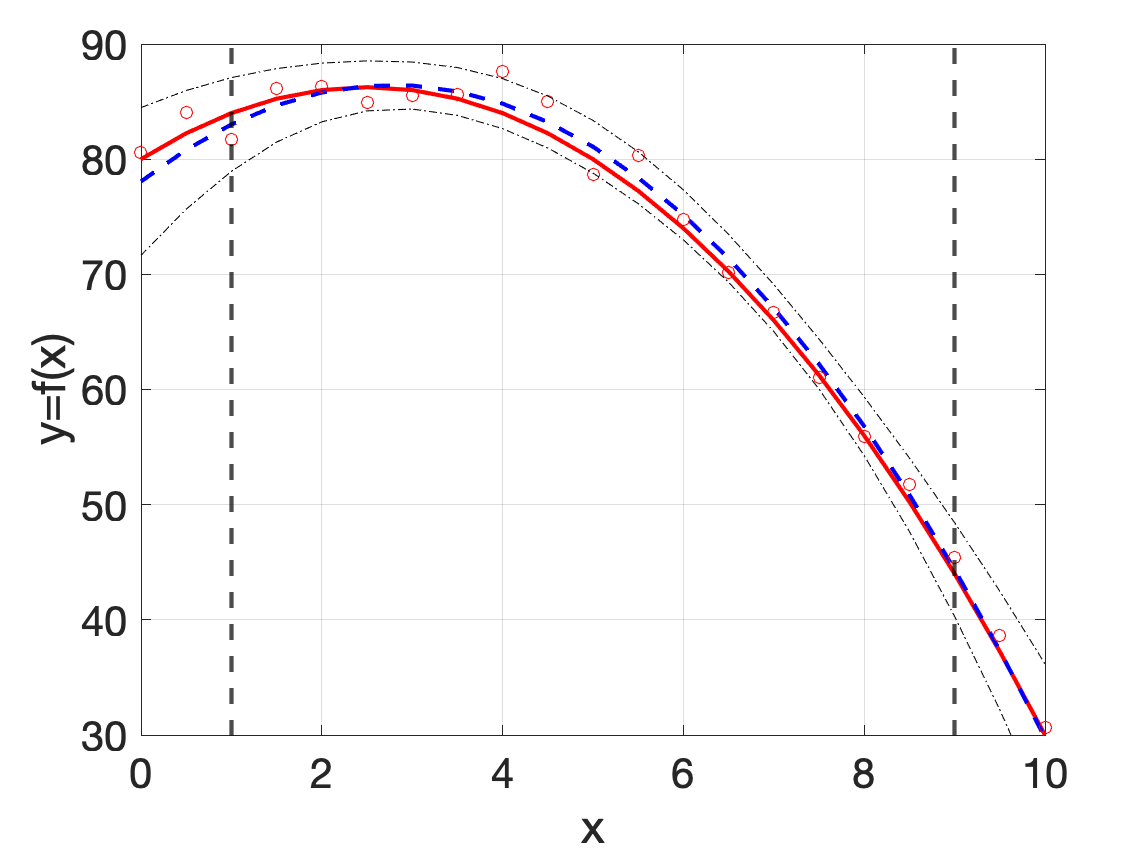
\includegraphics[width=0.7\linewidth]{sovra-a} \caption{}
			\end{subfigure}
			\begin{subfigure}{0.49\linewidth}
				\centering
				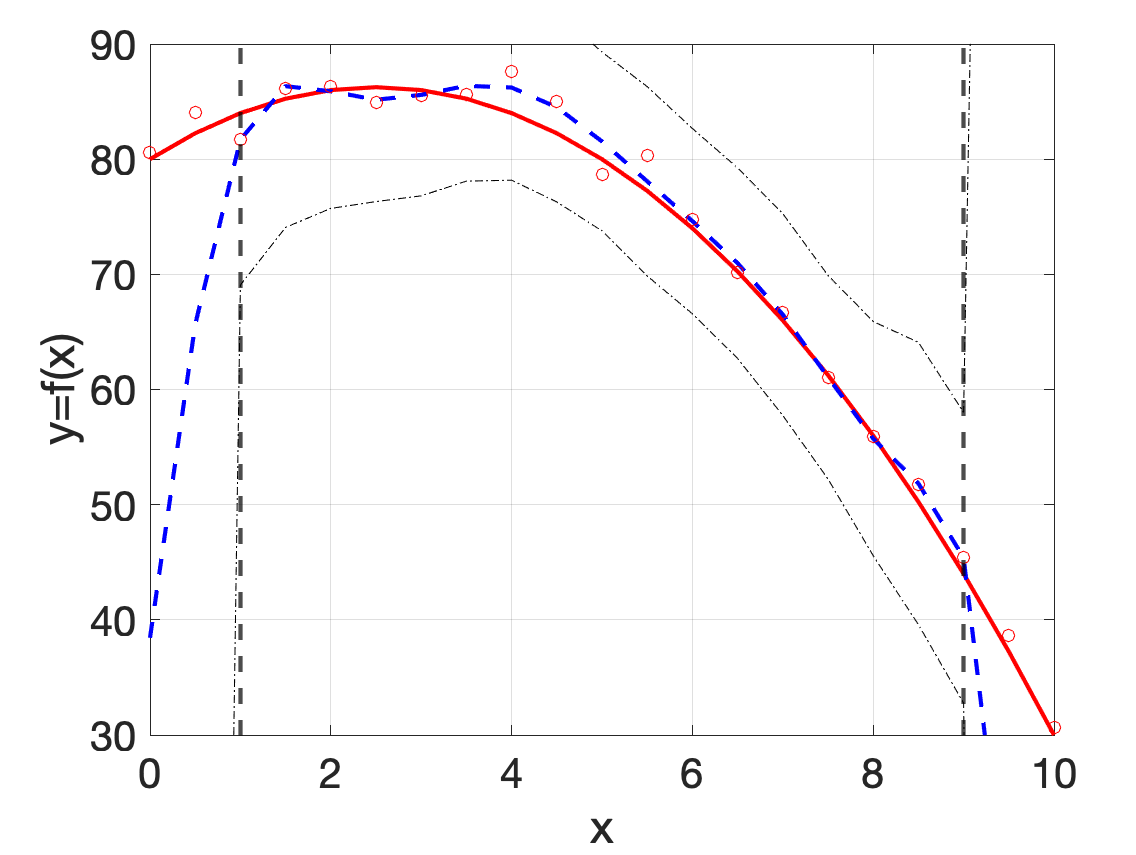
\includegraphics[width=0.7\linewidth]{sovra-b} \caption{}
			\end{subfigure}
			\caption{regressione di un campione di origine quadratica (linea rossa) tramite un polinomio di secondo grado (a) e di nono grado (b) rappresentati dalle linee tratteggiate blu.}
			\label{fig:stat:sovraadattamento}
		\end{figure}
	
\section{Taratura statica}
	La \de{taratura} di uno strumento di misura è l'identificazione della correlazione tra il misurando (il predittore $x$ della regressione) con l'uscita (risposta $y$) dello strumento stesso. La \de{taratura statica} è dunque effettuata in condizioni statiche, ossia assumendo che né misurando né uscita dello strumento siano funzioni del tempo, ma che siano costanti nello stesso.
	
	La correlazione $y=f(m)$ tra ingresso $m$ e uscita $y$ in condizioni statiche è detta \de{caratteristica statica} dello strumento. In generale uno strumento di misura operante in condizioni statiche fornisce una misura mediante l'inversione della caratteristica statica: nota infatti la caratteristica e il valore osservato dall'uscita $y_0$ è possibile ottenere per inversione la stima del misurando $m_0$.	
	
	\figura{5}{1.5}{tarstat-b}{stima del misurando ottenuta tramite inversione della caratteristica statica sfruttando l'uscita osservata dallo strumento.}{tarstat}
	
	Nella fase di \textbf{taratura} in generale la \textbf{caratteristica statica} è \textbf{ignota} ed è dunque necessario utilizzare una serie di valori noti del misurando $m_i$ per determinare le uscite attese $y_i$ in modo da \textit{costruire} la caratteristica statica del modello mediante un'opportuna regressione.
	
	\figura{5}{1.5}{tarstat}{determinazione della caratteristica statica come regressione di misurandi noti e rispettive uscite.}{tarstat}
	
	Durante la fase di taratura è necessario che i misurandi $m_i$ siano:
	\begin{itemize}
		\item dei \textbf{campioni di riferimento} fondamentali per la grandezza in esame (come per esempio un set di masse di valore noto);
		\item campioni/ingressi generici misurati con uno \textbf{strumento di riferimento}.
	\end{itemize}
	In entrambi i casi è necessario imporre che l'accuratezza del campione/strumento di riferimento sia di almeno un ordine di grandezza superiore rispetto all'accuratezza del sistema di misura da tarare.
	
	Con la fase di taratura è dunque possibile determinare sia la caratteristica statica del sistema, ma soprattutto l'incertezza della misura; in particolare nella fase di determinazione della caratteristica si trovano:
	\begin{itemize}
		\item lo sviluppo del modello dello strumento;
		\item la raccolta dei dati di taratura;
		\item l'analisi di regressione dei dati raccolti;
		\item la validazione della regressione mediante l'analisi dei residui.
	\end{itemize}
	Per quanto riguarda l'incertezza è necessario determinare le componenti:
	\begin{itemize}
		\item di incertezza sul modello;
		\item di incertezza sulla stima del misurando;
		\item di incertezza sulla curva di taratura.
	\end{itemize}
	
	\paragraph{Sviluppo del modello} Lo sviluppo del modello si basa sui principi di funzionamento dello strumento di misura, per questo è tipicamente analitico; esistono tuttavia modelli di origine numerica o semi-empirica.
	
	Un modello completo include, in generale, anche delle relazioni dovuti agli ingressi di disturbo (come per esempio le variazioni dovute alle temperatura) e di uscita sul sistema stesso; la differenza tra modello e realtà assume il nome di \de{incertezza di modello}.
	
	\figura{7}{0.66}{sisttar}{schema a blocchi di un sistema di misura}{sisttar}
	
	Considerando lo schema a blocchi di un sistema di misura in figura \ref{sisttar}, è possibile osservare che la misura è soggetta principalmente a due tipi di ingresso:
	\begin{itemize}
		\item l'\textbf{ingresso modificante} è un tipo di ingresso che influisce direttamente sul modello del sistema e dunque nella sua caratteristica statica. Sono degli ingressi più complessi da trattare e sono preponderanti quando il modello della misura è approssimato e non considera un effetto dominante (per esempio le variazioni di proprietà dovute alla temperatura) che possono comportare tarature errate; per limitare questo tipo di problema tendenzialmente si esegue una sequenza di test casualizzata (ossia non si incrementano gradualmente i campioni di riferimento, ripetendo misura più volte, ma si continua a cambiare casualmente il misurando, in modo da distribuire più uniformemente gli errori);
		\item l'\textbf{ingresso interferente} invece è dovuto ai disturbi casuali (tendenzialmente molto piccoli) che si sommano all'uscita del modello; essi possono essere ridotti in fase di taratura effettuando più test (in tempi diversi) a misurandi (ossia ingressi ad effetti dominanti) costanti, permettendo dunque di considerare tali fluttuazioni come distribuite normalmente per via del teorema del limite centrale: questa operazione prende il nome di \de{controllo statico}.
	\end{itemize}
	
	\textbf{VOLENDO SI PUò AGGIUNGERE ESEMPIO}
	
\section{Analisi di incertezza}
	Secondo la norma \texttt{UNI 4546} una \de{misura}, che rappresenta un parametro di un sistema considerato in un suo determinato stato, è composta da una triade di elementi: il \textbf{valore}	(nell'esempio che segue $35.2$), la sua \textbf{incertezza} ($0.1$) e l'\textbf{unità di misura} ($m$) associata alla misurazione nella forma
	\[ 35.2 \pm 0.1 m \]
	
	\paragraph{Incertezza  e GUM} Il concetto di \de{incertezza} è definito tramite la norma \texttt{UNI-CEI-ENV 13005} delle \de{GUM} (\textit{Guide to Uncertainty in Measurement}); questa normativa sostituisce il vocabolario precedente ridefinendo l'errore come \textbf{incertezza} e il valore vero con il termine \textbf{stima}.
	
	L'incertezza si riferisce solamente alla componente stocastica (casuale e non prevedibile) della misura. Per normativa infatti le componenti di deviazioni sistematica (gli ingressi interferenti laddove possibile) della misura devono essere corretti prima di riportare la misura stessa. Se tali effetti sono ignoti, allora essi possono essere considerati nella componente stocastica anche se il loro impatto risulterà essere maggiore (questa operazione è consentita solamente se, nella fase di taratura, si effettuano dei test casualizzati).
	
	L'\de{incertezza tipo} (\textit{standard uncertainty}) $u_x$ della variabile stocastica $x$ è definita come la deviazione standard del valor medio di $x$; ricordando dunque che $V(\ov x) = s_x^2/n$, allora è possibile osservare che l'incertezza tipo è definita come
	\begin{equation}
		u_x = \frac{s_x}{\sqrt n} = \sqrt{ \frac{\sum_{i=1}^n \big(x_i-\ov x\big)^2}{n(n-1)}}
	\end{equation}
	L'\de{incertezza relativa} $u_{x,\textrm{rel}}$ esprime invece l'incertezza come rapporto adimensionale tra incertezza tipo $u_x$ e valor medio campionario misurato (in modulo):
	\begin{equation}
		u_{x,\textrm{rel}} = \frac{u_x}{|\ov x|}
	\end{equation}
	\begin{nota}
		L'incertezza relativa è utilizzata tendenzialmente per confrontare valori di misurando molto differenti in quanto esprimono la deviazione standard in funzione del misurando stesso.
	\end{nota}
	In generale l'incertezza relativa $u_{x,\textrm{rel}}$ è molto piccola e si indica con una sola cifra significativa e si usano 3 notazioni principalmente: notazione scientifica ($7\cdot 10^{-5}$), parti per mille ($0.7 ^o/_{oo}$) o parti per milione ($70ppm$).
	
	\subsection{Intervalli di confidenza}
		In generale è utile esprimere l'incertezza come un intervallo all'interno del quale è probabile che ricada il valore atteso della popolazione da cui è estratto il campione dei valori di misura osservati: tale intervallo, analogo a come visto per la regressione (pag. \pageref{sec:stat:regrpred}), è detto \de{intervallo di confidenza} e la relativa probabilità associata è detta \de{livello di confidenza}.
		
		\vspace{3mm}
		Come visto a pagina \pageref{sec:stat:teststudent} tramite il test di student è possibile definire la statistica di test $t_0$ (che si distribuisce come una distribuzione T di Student) noto un campione $\langle x_i\rangle$ di media campionaria $\ov x$ e deviazione standard $s_x$ rispetto alla popolazione di valore atteso $\mu_0$ come
		\[ t_0 = \frac{\ov x - \mu_0}{s_x / \sqrt n} \backsim t_n\]
		
		Conoscendo la distribuzione della statistica di test $t_0$, allora la probabilità che la stessa ricada con una probabilità $1-\alpha$ (dove $\alpha$ è il $\pval$ della statistica) in tale distribuzione può essere determinata in funzione del quantile di probabilità $\alpha_2$ della T di Student di ordine $n$ indicato come $t_{n,\alpha/2}$:
		\begin{align*}
			P\left(-t_{n,\alpha/2} < \frac{|\ov x - \mu 0|}{s_x/\sqrt n} < t_{n,\alpha/2} \right) & = 1-\alpha  \\			
			\xrightarrow{s_{x}/\sqrt n \rightarrow u_x} \qquad P \Big(\ov x - t_{n,\alpha/2} u_x < \mu_0  < \ov x + t_{n,\alpha/2} u_x\Big) & = 1- \alpha
		\end{align*}
		
		E' dunque possibile affermare che l'intervallo di estremi $\ov x \pm t_{n,\alpha/2}u_x$ è proprio l'intervallo all'interno del quale ricade il valore atteso con un \textbf{livello di confidenza} pari a $1-\alpha$. \\
		Essendo $s_x /\sqrt n$ pari all'incertezza tipo e definendo il quantile $t_{n,\alpha/2} = k_n$ il \textbf{fattore di copertura} (dipendente dalla dimensione del campione $n$) è possibile definire l'\de{incertezza estesa} $U_x$ della misura come
		\[ U_x = t_{n,\alpha/2} \frac{ s_x}{\sqrt n} = k_n \, u_x\]
		
		Di fatto il fattore di copertura $k_n$ permette di stabilire di quanto debba essere moltiplicata l'incertezza tipo per avere un'affidabilità pari a $1-\alpha$ in funzione del numero di campioni $n$ analizzati e a tal fine si utilizza generalmente la funzione CDF.
		\begin{nota}
			Per un numero di campioni $n>20$ la distribuzione T di Student può essere approssimata ad una distribuzione normale e dunque si può utilizzare la sua CDF.	
		\end{nota}
		In tabella \ref{tab:stat:copertura} è possibile osservare per alcuni fattori di confidenza $k$ il livello di confidenza associato.
		\begin{SCtable}[1.5][bht]
			\centering
			\begin{tabular} {c | c}
				$\quad k \quad $ & copertura $= 2f_{cd,l}(k)-1$ \\ \hline
				1 & 68.27\% \\
				1.645 & 90\% \\
				1.960 & 95\% \\
				2 & 95.45\% \\
				2.576 & 99\% \\
				3 & 99.73\%
			\end{tabular}
			\caption{livello di confidenza associato al fattore di copertura $k$.} \label{tab:stat:copertura}
		\end{SCtable}
	
	\subsection*{Incertezza ex-post}
		L'incertezza sui dati può anche essere calcolata ex-post, ossia su dati ottenuti da un sistema di misura di cui è nota l'incertezza e viene espressa in \textbf{intervallo di predizione} (associato alla probabilità che le nuove osservazioni rientrino in tale fascia) e \textbf{intervallo di confidenza} (associato alla probabilità rispetto alla quale ci si attende che il valor atteso della popolazione ricada).
	
	\subsection{Incertezza tipo e incertezza estesa}
		Salvo diverse indicazioni per le misurazioni si utilizza l'\de{incertezza tipo}, ossia seguendo la dicitura
		\[ 27.5 \pm 0.1mm \]
		allora il termine $0.1$ è associato all'incertezza tipo $u_x = 0.1$. E' altresì possibile utilizzare l'\de{incertezza estesa} aggiungendo alla misura il livello di confidenza associato all'incertezza tipo riportata con una dicitura del tipo
		\[ 27.5\pm 0.1 mm \quad \textrm{con confidenza al 99\%} \]
	
	
	
	
	
	
	
	
	
	
	\chapter{Misura di spostamento}

\section{Encoder ottici}

\section{Potenziometro}
	Il \de{potenziometro} è un trasduttore della misura ingresso-spostamento che viene trasdotta in una tensione elettrica; il moto dei corpi Potenziometroviene caratterizzato dalle grandezze di spostamento, velocità e accelerazione (le ultime possono essere ricavate per derivazione). Essi permettono inoltre di misurare degli spostamenti sia assoluti che relativi, ma anche di tipo lineare o angolare.
	
	I \textbf{potenziometri} possono essere a \de{traslazione} che si basano sulla traslazione di un cursore, il potenziometro a \de{rotazione ad un giro} (analogo a quello di traslazione che tuttavia misura variazioni angolari) e \de{a rotazione ad elica} (permette di misurare più giri).
	
	\paragraph{Potenziometro rotativo} \textbf{FIGURA}
	
	Un potenziometro rotativo è un componente a 3 \textit{pin}: i due più esterni sono collegati alla tensione di alimentazione, mentre il pin centrale presenta la tensione in uscita ottenuta dal partitore di tensione della resistenza interna del potenziometro.
	
	La resistenza interna è tendenzialmente realizzata da polveri ceramiche/plastiche. Il modello ideale del potenziometro è dunque quello del partitore di tensione la cui somma delle resistenze è pari alla resistenza nominale $R_p$. La ripartizione della resistenza complessiva dipende dunque dalla posizione del cursore dipendente dal misurando del sistema.
	
	Nota la lunghezza $L$ della corsa e la posizione $x$ del cursore, allora il partitore è composto dalle resistenze
	\[ R_1 = R_p \frac{L-x}{L} \qquad R_2 = R_p \frac x L\]
	Dall'equazione del partitore (dove $V_{dd}$ è la tensione di alimentazione del circuito) è possibile scrivere la tensione in uscita nel caso ideale come 
	\begin{equation} \label{eq:pot:ideale}
		V_{out}= V_{dd} \frac{R_2}{R_1+R_2} = V_{dd} \frac{x}{L-x+x} = V_{dd} \frac x L
	\end{equation}
	
	Il modello ottenuto è lineare, tuttavia facendo la taratura di un sistema reale si osserva uno scostamento dal caso ideale che può essere tuttavia modellato da una resistenza $R_m$ che rappresenta il carico esterno (dovuta all'oggetto che effettua la misurazione della tensione).
	
	\textbf{INSERIRE SCHEMA MODELLO REALE} 
	
	A questo punto il partitore di tensione è dato dalla resistenza $R_1$ e dal parallelo di $R_2$ con $R_m$ pari a 
	\[ R_2 \parallel R_m = \frac{R_mR_p \frac x L}{R_m + R_p \frac x L} \qquad\]
	Questo permette di ottenere un nuovo modello che considera anche la resistenza di carico $R_m$ come
	\[ V_{out} = V_{dd} \frac{R_2\parallel R_m}{ R_1 + R_2\parallel R_m} = V_{dd} \frac{x/L}{1 + \dfrac{R_p}{R_m} \dfrac{x}{L} \left(1 - \dfrac x L\right)   } \]
	A questo punto è possibile osservare che un modello più realistico non è più lineare (rispetto al misurando $x$) come il modello ottenuto in prima battuta in equazione \ref{eq:pot:ideale}. In particolare nel caso in cui $R_m \rightarrow \infty$ (resistenza di carico infinita) allora il comportamento risulterebbe essere approssimato al caso ideale con caratteristica di uscita lineare. Un altro modo per ottenere valori reali \textit{simili} al comportamento ideale sarebbe quello di avare una resistenza complessiva $R_p$ tendente a zero (richiesta che si scontra con la realizzazione pratica dei potenziometri reali).
	
	\textbf{FIGURA DEL COMPORTAMENTO REALE}
	
	In particolare il problema di scegliere un valore $R_p$ si ottiene una sensibilità bassa in quanto sarebbe limitata  la tensione $V_{dd}$ di alimentazione del meccanismo. Ogni resistenza può infatti dissipare una potenza massima $P$, ed essendo che la caduta di tensione alla stessa $V$ allora si ricava che
	\[P = \frac{V^2}{R_p} \qquad \Rightarrow \quad V = \sqrt{PR_p}\]
	Dunque se $R_p$ piccolo, allora necessariamente $V_{dd}$ è bassa: questo porta ad un'abbassamento della pendenza della caratteristica di uscita che diminuisce la sensibilità del sistema. Inoltre il problema è anche termico in quanto se la potenza da dissipare è eccessiva, il dispositivo potrebbe andare incontro a rottura.
	
	\textbf{FARE TABELLA DEL PERCHÈ SI SCEGLIE RP}
	
	\paragraph{Sensibilità al contatto} Un possibile problema del funzionamento del potenziometro è quello dovuto alla sensibilità del contatto dovuto alle vibrazioni meccaniche. Per eliminare questo problema è possibile immergere il cursore nell'olio (che funge da smorzatore di oscillazioni) oppure equipaggiare il potenziometro con due testine con modi di vibrazione disaccoppiati.
	
	
	
	
	
	
	
	
	
	
	
	
	
	
	
	
	
	
	
	
	
	\chapter{Misure dinamica}
	La \de{dinamica} tratta la misurazione di entità tempo varianti utilizzando la \de{trasformata di Fourier}.
	
\section{Trasformata di Fourier}
	
	\paragraph{Analogia con il caso vettoriale} La trasformata di Fourier può essere analizzata effettuando un'analogia con la scomposizione di un vettore $\ov v$ (nel piano) nelle sue due componenti; noti i versori della terna ortonormale $\ov e_1,\ov e_2$, il vettore $\ov v$ può essere espresso come una combinazione vettoriale del tipo
	\begin{equation} \label{eq:four:vettcombinazione}
		\ov v = \alpha \ov e_1 + \beta \ov e_2
	\end{equation}
	A questo punto è necessario determinare i valori dei coefficienti $\alpha,\beta$ che rappresentano le coordinate di $\ov v$ nella base dei vettori $\ov e_1,\ov e_2$: questo a livello vettoriale può essere effettuato considerando il prodotto scalare tra vettori come segue
	\begin{equation} \label{eq:four:vettcoordinate}
		\alpha = \ov v \cdot \ov e_1 \qquad \beta = \ov v \cdot \ov e_2 \qquad \Rightarrow \quad \ov v = \big(\ov v \cdot \ov e_1\big) \ov e_1 + \big(\ov v\cdot \ov e_2\big) \ov e_2
	\end{equation}
	A questo punto il vettore $\ov v$ nel sistema di riferimento associato può essere scritto come una $2-$upla composta dalle sue coordinate nella base associata:
	\begin{equation} \label{eq:four:vettrappresentazione}
		\ov v = \begin{bmatrix}
			 \alpha \\ \beta
		\end{bmatrix}
	\end{equation}
	
	\paragraph{Sviluppo in serie} Lo \de{sviluppo in serie di Fourier} permette di rappresentare un segnale periodico $g(t)$ di periodo $T$ tramite un'opportuna sovrapposizione di segnali (co)sinusoidali con frequenza multipla all'\de{armonica fondamentale} $f_0 = 1/T$:
	\begin{equation} \label{eq:four:serie1}
		g(t) = \frac 1 2 a_0 + \sum_{n=1}^\infty a_n \cos\big(\omega_n t\big) + \sum_{n=1}^\infty b_n\sin\big(\omega_n t\big) \qquad \textrm{con } \omega_n = 2\pi f_0
	\end{equation}
	
	Questa equazione può dunque essere pensata per analogia alla scomposizione vettoriale (eq. \ref{eq:four:vettcoordinate}) dove le componenti $a_i,b_i$ sono associati ai vari segnali (co)sinusoidali che si dimostrano formare una \textbf{base ortogonale}.
	\begin{dimostrazione}
		Per dimostrare l'ortogonalità della base formata dai segnali (co)sinusoidali con frequenze armoniche multiple della fondamentale è necessario definire i prodotto scalare tra due funzioni periodiche $g(t)$ e $f(t)$ (di pari periodo $T$) definito come
		\[ g(t) \cdot f(t) = \frac 1 T \int_0 ^T g(t) \, f^*(t) \, dt  \]
		dove con $f^*(t)$ si intende la funzione complessa coniugata di $f(t)$ che nel caso di funzioni reali coincide con la funzione stessa (dunque in questo caso $f^*(t) = f(t)$). 
		
		Introducendo questa definizione di prodotto scalare è possibile pensare di calcolare la trasformata della funzione $g(t)$ come il prodotto scalare tra le sue coordinate per le basi dello spazio (co) sinusoidali (similarmente ai risultati ottenuti in figura \ref{eq:four:vettcoordinate}):
		\[ g(t) = \frac 1 2 a_0 + 2 \sum_{n=1}^\infty \Big[ g(t) \cdot \cos(\omega_nt) \Big]  \cos(\omega_nt) + 2 \sum_{n=1}^\infty \Big[g(t)\cdot \sin(\omega_nt)\Big]\sin(\omega_nt) \]
		
		Questa relazione risulta essere verificata in quanto effettuando i seguenti prodotti scalari tra le componenti della base ortonormale si ottengono le seguenti uguaglianze:
		\begin{itemize}
			\item $\sin\big(\omega_n t\big) \cdot \sin(\omega_n t) = 1$ 
			\item $\cos\big(\omega_n t\big) \cdot \cos(\omega_n t) = 1$ 
			\item $\sin\big(\omega_n t\big) \cdot \cos(\omega_n t) = 0$ 
			\item $\sin\big(\omega_n t\big) \cdot \sin(\omega_j t) = 0$ per ogni $i\neq j$
			\item $\cos\big(\omega_n t\big) \cdot \cos(\omega_j t) = 0$ per ogni $i\neq j$
		\end{itemize}
		Attenzione che il prodotto scalare tra i coseni è definito precedentemente e prevede di fatto di effettuare una media integrale sul periodo del prodotto delle due funzioni (co)sinusoidali! Per questo ci sono termini che si annullano o che risultano avere media integrale unitaria.
		
	\end{dimostrazione}

	A questo punto è possibile definire un'operazione analoga all'equazione \ref{eq:four:vettcoordinate} per determinare le componenti $a_n,b_n$ della serie di Fourier nella base dei segnali (co)sinusoidali che risulta valere
	\begin{equation} \label{eq:four:temp2}
		a_n = \frac 2 T \int_0^T g(t) \cos\big(\omega_n t\big) \, dt \qquad b_n = \frac 2 T \int_0^T g(t) \sin\big(\omega_n t\big) \, dt
	\end{equation}
	
	\textbf{RIVEDERE LA DIMOSTRAZIONE}
	
	L'insieme discreto delle coordinate $a_n,b_n$ che compongono la trasformata di Fourier del segnale periodico $g(t)$ possono dunque essere rappresentate in appositi diagrammi come in figura \ref{four-ab}.
	
	\figura{3}{2}{four-ab}{diagramma delle coordinate ottenute dalla trasformata di Fourier di una funzione $g(t)$. }{four-ab}
	
	
	\subsection{Formulazione tramite fasori}
	La trasformata di Fourier può altresì essere espressa attraverso una formulazione fasoriale; considerando la \de{formula di Eulero} per la quale $e^{i\omega t}$ (dove $i$ è la costante immaginaria pari a $\sqrt{-1}$) può essere espresso come la somma di un seno e un coseno immaginario secondo la relazione $\cos(\omega t) + i\sin(\omega t)$, allora è possibile riscrivere le basi per la scomposizione tramite Fourier con le equazioni
	\[ \cos\big(\omega_n t\big) = \frac{e^{i\omega_nt} + e^{-i\omega_n t}}{2} \qquad \sin\big(\omega_n t\big) = \frac{e^{i\omega_nt}-e^{-i\omega_nt}}{2i} \]
	
	Utilizzando queste relazioni nell'equazione \ref{eq:four:serie1} è possibile riscrivere la trasformata di Fourier come
	\begin{equation} \label{eq:four:temp1}
		\begin{split}
		g(t) & = \frac 1 2 a_0 + \sum_{i=0}^\infty a_n \frac{e^{i\omega_n t} + e^{-i\omega_n t}}{2} + \sum_{i=0}^\infty b_n \frac{e^{i\omega_n t} - e^{-i\omega_n t}}{2i} \\
		& = \frac 1 2 a_0 + \frac 1 2 \sum_{n=1}^\infty \big(a_n - i b_n\big)e^{i\omega_nt} + \frac 1 2 \sum_{n=1}^\infty \big(a_n + i b_n\big) e^{-i\omega_nt}
		\end{split}
	\end{equation}
	
	A questo punto è possibile pensare che la base della scomposizione della funzione periodica $g$ possa essere determinata dai fasori $e^{j\omega_nt}$ e $e^{-j\omega_nt}$ rispetto ai quali le coordinate sono espresso dal numero complesso determinati dalle coppie $a_n \pm i b_n$. A questo punto è possibile pensare di ridefinire tali parametri in funzione dei fasori $G_n$ definiti come
	\[G_0 = \frac 1 2 a_0 \qquad G_n = \frac 1 2 \big(a_n - ib_n\big) \qquad G_{-n} = \frac 1 2 \big(a_n + ib_n\big) = G^*_n\]
	E' possibile dunque osservare la relazione che intercorre tra i coefficienti fasoriali $G_n$ con $n$ positivo e negativo: in particolare i coefficienti a pedice negativo coincidono con la rispettiva coordinata coniugata ($^*$ indica l'operatore coniugio). Utilizzando questa relazioni è possibile riscrivere la trasformata di Fourier (eq. \ref{eq:four:temp1}) in maniera più compatta come	
	\begin{equation}
	g(t) = G_0 + \sum_{n=1}^\infty G_n e^{i\omega_n t} + \sum_{n=-1}^{-\infty} G_{n} e^{i\omega_n t} =  \sum_{n=-\infty}^{+\infty} G_n e^{j\omega_n t} 
	\end{equation}
	
	Utilizzando una notazione fasoriale per l'espressione della serie di Fourier è dunque necessario riscrivere l'equazione \ref{eq:four:temp2} per il calcolo delle coordinate delle funzione nella nuova base dei fasori $e^{i\omega_n t}$; utilizzando la definizione del prodotto scalare definita in precedenza le componenti $G_n$ si ricavano come
	\[ G_n = g(t) \cdot e^{j\omega_nt}= \frac 1 T \int_0^T g(t) \cdot \left(e^{j\omega_n t} \right)^*\ \, dt\ = \frac 1 T \int_0^T g(t) e^{-j\omega_n t} , dt\]
	Questa funzione può essere rappresentata più facilmente rappresentando in due diagrammi il modulo e la fase dei fasori nel segnale.
	
	\textbf{RIVEDERE LA LEZIONE}
	
	\paragraph{Trasformata di una funzione senza periodo} Una funzione che non ha periodo può essere modellata come una funzione di periodo infinito $T\rightarrow \infty$ (o periodo associato al tempo di misurazione del segnale).
	Considerando il coefficiente $A_n$ definito come
	\[A_n : = G_n T = \int_0^T g(t) e^{-j\omega_nt}\, dt\]
	allora è possibile riscrivere la trasformata di Fourier come
	\[ g(t) = \frac 1 T \sum_{n=-\infty}^\infty A_n e^{j\omega_n t} \]
	Ponendo $T\rightarrow \infty$ allora è possibile calcolare i coefficienti $A_n$ come
	\[A_n \xrightarrow{T\rightarrow\infty} \int_0 ^\infty g(t)e ^{-j\omega_nt}\, dt \qquad \Rightarrow g(t) \xrightarrow{T\rightarrow \infty} \int_0^\infty A(\omega) e^{i\omega_n t} \underbrace{\frac 1 T}_{df} = \int_0^\infty A(\omega) e^{i\omega t}\, df = \frac 1 {2\pi}\int_0^\infty G(\omega) e^{i\omega t}\, d\omega \]
	
	
	\begin{concetto}
		La \de{trasformata di Fourier} permette dunque di ricavare la funzione $G(\omega)$ nel dominio delle frequenze partendo dalla funzione $g(t)$ espressa nel dominio del tempo:
		\begin{equation} \label{eq:four:trasformata}
			G(\omega) = \int_{-\infty}^{\infty} g(t) e^{-i\omega t} \, dt
		\end{equation}
		L'\de{antitrasformata di Fourier} invece permette di svolgere l'operazione inversa, ossia nota la funzione $G(\omega)$ nel dominio della frequenza è possibile ricavare la funzione $g(t)$ tramite l'equazione
		\begin{equation} \label{eq:four:antitrasformata}
			g(t) = \frac 1 {2\pi} \int_{-\infty}^\infty  G(\omega) e^{-i\omega t}\, d\omega
		\end{equation}
	\end{concetto}
	
	\subsection{Proprietà della trasformata di Fourier} 
		La \de{trasformata di Fourier} è un'operatore \de{lineare}, ossia una funzione $g(t)$ ottenuta come combinazione lineare di funzioni più semplici $f_i$ può essere trasformata ricombinando egualmente le trasformate delle funzioni $f_i$; la linearità può essere modellata dalla relazione
		\[  \alpha x_1 + \beta x_2 \quad \mapsto \quad \alpha X_1 + \beta X_2 \]
		\begin{dimostrazione}
			Per dimostrare la linearità della trasformata di Fourier è sufficiente considerare il seguente esempio:
			\begin{align*}
				\four{a\, x(t) + b\, y(t)} & = \int_{-\infty}^\infty \Big( a\, x(t) + b\, y(t)\Big) e^{-i\omega t} dt \\
				& = a \int_{-\infty}^\infty x(t)e^{-i\omega t} \, dt + b \int_{-\infty} ^\infty y(t)e^{-i\omega t}\, dt \\
				& = a \,X(\omega) + b\, Y(\omega)
			\end{align*}
		\end{dimostrazione}
		
		
		Tra le \de{proprietà} fondamentali della trasformata di Fourier troviamo la regola sia di \de{derivazione} che di \de{integrazione} per un segnale $x(t)$ nel dominio del tempo; nota infatti la sua trasformata $X(\omega)$ è possibile verificare le seguenti proprietà:
		\begin{equation} \label{eq:four:derivata7}
			\begin{split}
				\textrm{derivazione:} \qquad \frac d{dt}x(t) \quad & \mapsto \quad i\omega X(\omega)\\
				\textrm{integrazione:} \qquad\int x(t)\, dt \quad & \mapsto \quad \frac 1 {i\omega} X(\omega)
			\end{split}
		\end{equation}
		Questa proprietà è particolarmente utile in quanto permette di trasformare le equazioni differenziali lineari nel dominio del tempo in equazioni algebriche nel dominio della frequenza.
		\begin{dimostrazione}
			La proprietà associata alla derivata può essere dimostrata derivando nel tempo la relazione esplicita dell' antitrasformata di Fourier (eq. \ref{eq:four:antitrasformata}):
			\begin{align*}
				\frac d {dt} x(t) & = \frac d {dt} \left(\frac 1 {2\pi} \int_{-\infty}^\infty  X(\omega) e^{-i\omega t}\, d\omega\right) = \frac 1{2\pi} \int_{-\infty}^\infty X(\omega) \, \frac d{dt}\left(e^{i\omega t}\right) \, d\omega \\ &  = \frac 1 {2\pi} \int_{-\infty}^\infty i\omega\, X(t\omega) e^{i\omega t}\, d\omega = \antif{i\omega \, X(\omega)}
			\end{align*}
		\end{dimostrazione}
		
		Altre \de{proprietà} utili per effettuare trasformazioni di funzioni dal dominio del tempo al dominio della frequenza (e viceversa) sono quelle di \de{convoluzione} e del \de{prodotto} definite come 
		\begin{align*}
			\textrm{convoluzione:} \qquad x(t) \otimes y(t) \quad & \mapsto \quad X(\omega) \, Y(\omega)\\
			\textrm{integrazione:} \qquad\int x(t)\, y(t) \quad & \mapsto \quad X(\omega) \otimes Y(\omega)
		\end{align*}
		La \textbf{convoluzione}, denotata dall'operatore matematico $\otimes$, di due funzioni è definita dall'espressione:
		\[ x(t) \otimes y(t) = \int_{-\infty}^\infty x(\tau) y(t-\tau)\, d\tau  \]
		
		\begin{dimostrazione}
			La dimostrazione della proprietà di convoluzione si effettua applicando la definizione dell'operatore $\otimes$ all'espressione della trasformata di Fourier (eq. \ref{eq:four:trasformata}):
			\begin{align*}
				\four{x(t)\otimes y(t)} & = \int_{-\infty}^\infty \left( \int_{-\infty}^\infty x(\tau) y(t-\tau) \, d\tau\right) e^{-i\omega t}\, dt \\
				& = \int_{-\infty}^\infty x(\tau) \left(\int_{-\infty}^\infty y(t-\tau) e ^{-i\omega t} \, dt\right)\, d\tau
			\end{align*}
			Effettuando la trasformazione delle coordiante $\xi = t-\tau$ (da cui $t= \xi + \tau $ e  $d\xi = dt$) per facilitare il calcolo integrale, è possibile concludere la dimostrazione come
			\begin{align*}
				\four{x(t)\otimes y(t)} & = \int_{-\infty}^\infty x(\tau) \left( \int_{-\infty}^\infty y(\xi) e^{-i\omega \xi} e^{-i\omega \tau}\, d\xi \right)\, d\tau \\
				& = \int_{-\infty}^\infty x(\tau) e^{-i\omega \tau} \left( \int_{-\infty}^\infty y(\xi) e^{-i\omega \xi}\, d\xi\right) \, d\tau \\
				& = \int_{-\infty}^\infty x(\tau) e^{-i\omega \tau} Y(\omega) \, d\tau \\
				& = X(\omega)\, Y(\omega)
			\end{align*}
		\end{dimostrazione}
		
		E' possibile utilizzare anche la \de{proprietà} di \de{traslazione nel tempo}, ossia nota una funzione $x(t)$ nel dominio del tempo e la sua rispettiva trasformata $X(\omega)$, la trasformata di della funzione $x(t-\tau)$ (con $\tau$ una costante qualsiasi di traslazione temporale) può essere determinata come
		\[ x(t-\tau) \quad \mapsto \quad X(\omega) e^{-i\omega \tau} \]
		Analoga a questa proprietà è quella della \de{modulazione} che permette di stabilire l'antitrasformata di uno spettro traslato di una pulsazione $\omega_0$:
		\[ x(t) e^{-i\omega_0t} \quad \mapsto \quad X(\omega-\omega_0) \]
		
		\begin{dimostrazione}
			Si può dimostrare la traslazione nel dominio del tempo $x(t + \tau)$ di un segnale applicando la definizione formale di trasformata di Fourier (eq. \ref{eq:four:trasformata}) effettuando lo scambio di variabile di integrazione $t' = t + \tau$ (che determina $dt' = dt$ in quanto $\tau$ è costante):
			\begin{align*}
				\four{x(t+\tau)} & = \int_{-\infty}^\infty x(t+\tau) e^{-i\omega t}\, dt = \int_{-\infty}^\infty x(t') e^{-i\omega (t'-\tau)} \, dt' \\
				& = e^{i\omega \tau} \int_{-\infty}^\infty x(t') e^{-i\omega t'} \, dt' \\
				& = X(\omega) e^{i\omega \tau}
			\end{align*}
		\end{dimostrazione}		
		Altre proprietà che attualmente non si dimostrano ma possono essere utili sono quelle di:
		\begin{align*}
			\textrm{dualità:}& \qquad X(t) \quad \mapsto \quad x(-\omega) \\
			\textrm{coniugazione:}& \qquad x^*(t) \quad \mapsto \quad X^*(-\omega) \\
			\textrm{variazione di scala:}& \qquad x(at) \quad \mapsto \quad \frac 1 {|a|} X\left(\frac \omega a\right) \\
		\end{align*}
		
	\subsection{Trasformata di un'equazione differenziale}
		
			Un vantaggio di utilizzare la \de{trasformata di Fourier} è che ci permette di \de{risolvere} agilmente \de{equazioni differenziali lineari}; considerando per esempio un'equazione differenziale lineare del secondo ordine, la sua formulazione generica uò essere ricondotta ad una  forma
			\[ \frac{d^2\,y(t)}{dt^2} + a \frac{d\, y(t)}{dt} + b\, y(t) = c\,u(t)\]
			dove $u(t)$ è l'ingresso \de{forzante} del sistema, mentre $y(t)$ è la \de{risposta} (uscita) del sistema che si sta analizzando. 
			
			Utilizzando la proprietà della derivata (eq. \ref{eq:four:derivata7}) dimostrata in precedenza, è possibile riscrivere le derivate della risposta del sistema nel dominio della frequenza come:
			\[ \frac{d\,y(t)}{dt}\mapsto i\omega Y(\omega) = G(\omega) \qquad  \frac{d^2\,y(t)}{dt^2}\mapsto i\omega G(\omega) = (i\omega)^2 Y(\omega)  \]
			A questo punto è possibile riscrivere l'equazione differenziale di partenza nel dominio della frequenza, osservando che essa è lineare in $\omega$ e dunque può essere opportunamente invertita per determinare $Y(\omega)$ in funzione dell'ingresso $U(\omega)$:
			\[  (i\omega)^2 Y(\omega) + i\omega a Y(\omega) + bY(\omega) = c U(\omega) \qquad \Rightarrow\quad Y(\omega) = \underbrace{\frac c {b + i\omega a + (i\omega)^2}}_{H(\omega)} U(\omega) \]
			
			E' dunque possibile affermare che la risposta $Y(\omega)$ del sistema è proporzionale secondo un fattore $H(\omega)$ (dipendente anch'esso dalla pulsazione $\omega$) all'ingresso $U(\omega)$; in particolare la funzione complessa $H(\omega)$ prende il nome di \de{funzione di trasferimento}.
			
			In generale l'uscita di un sistema di equazioni differenziali lineari si può dunque esprimere in due maniere distinte, seppur analoghe, in funzione del dominio nel quale si sta analizzando:
			\begin{itemize}
				\item nel dominio della frequenza è possibile considerare la risposta come la moltiplicazione della trasformata dell'ingresso $U(\omega)$ per una funzione di trasferimento complessa $H(\omega)$;
				\item nel dominio del tempo la risposta si può valutare come al convoluzione tra l'ingresso $x(t)$ e l'antitrasformata della funzione di trasferimento (che dimostreremo rappresentare la risposta del sistema ad un impulso ideale).
			\end{itemize}
			
			\paragraph{Funzione di trasferimento come risposta ad un impulso} E' possibile affermare che la funzione di trasferimento rappresenta la risposta del sistema che si sta analizzando se sottoposto ad un impulso ideale. Per dimostrare questa affermazione è necessario introdurre il \textbf{\textit{delta} di Dirac} $\delta(t-t_0)$, ossia una particolare funzione che vale infinito nel tempo $t= t_0$ mentre è nulla in tutti gli altri punti; per definizione il picco e l'intervallo $dt$ dell'impulso sono infinitesimi dello stesso ordine tali che
			\[ \int_{-\infty}^\infty \delta\big(t-t_0\big)\, dt = 1 \qquad \forall t_0 \]
			
			Trasformando con Fourier la funzione $\delta$ si ottiene che la funzione $U(\omega) = \four{\delta} = 1$ assume valore costante unitario per qualsiasi frequenza $\omega$ cui è sottoposto il sistema; questo permette dunque di affermare che la risposta di un sistema lineare all'impulso coincide, nel dominio della frequenza, con la funzione di trasferimento:
			\[ \quad Y(\omega) = H(\omega) U(\omega) \quad \xrightarrow[U(\omega)=1 \ \forall \omega]{u(t) = \delta(t-t_0)} \quad Y(\omega) = H(\omega) \]
			
	\subsection{Funzione di trasferimento sinusoidale}
		
		Si consideri il caso di un sistema dinamico lineare del quale è nota la funzione di trasferimento $H(\omega)$; considerando di avere in ingresso una funzione puramente armonica sinusoidale del tipo $u(t) = \sin(\omega_0 t)$, lecito è chiedersi come si comporterà il sistema nel tempo, ossia valutare $y(t)$.
		\begin{nota}
			Questa analisi è molto importante; potendo infatti, tramite la serie di Fourier, approssimare ogni funzione ad una combinazione di segnali (co)sinusoidali, essendo il problema lineare è possibile utilizzare il principio di sovrapposizione degli effetti per calcolare l'uscita $y(t)$ antitrasformando le risposte di ogni componente armonica di $u(t)$.
		\end{nota}
		
		In primo luogo è dunque necessario determinare la trasformata $U(t)$ del segnale sinusoidale in ingresso; applicando la definizione si arriva dunque alla formulazione:
		\[U(\omega) = \int_{-\infty}^\infty \sin(\omega_0 t) e^{-i\omega t}\, dt = \int_{-\infty}^\infty \sin(\omega_0t) \Big(\cos(\omega t) + i\sin(\omega t)\Big) \, dt\]	
		Si osserva così che la trasformata di $\sin(\omega_0 t)$ è sempre nulla per ogni pulsazione $\omega \neq \pm \omega_0$ per via delle proprietà di ortonormalità della base di segnali (co)sinusoidali armonici; è dunque necessario determinare il valore dello spettro $U$ nei punti $\omega= \omega_0$ e $\omega = - \omega_0$ rispetto ai quali non è possibile stabilire a priori il valore della trasformata:
		
		\begin{align*}
			U(\omega_0) & = \int_{-\infty}^\infty\sin(\omega_0 t) (-i\sin(\omega_0 t)) \, dt = - i\int_{-\infty}^\infty \sin^2(\omega_0t) \, dt = - i\int_{-\infty}^\infty \frac {1-cos(2\omega_0 t)}2 \, dt \\
			& = - \frac i 2 \infty = -\frac  i 2 \, \delta(\omega - \omega_0)\\
			U(-\omega_0) & = \frac i 2 \infty = \frac i 2 \delta(\omega+\omega_0)
		\end{align*}
		A questo punto potendo esprimere la trasformata di  $u(t) = \sin(\omega_0t)$ nel dominio delle frequenze come $U(\omega) = \frac i 2 \delta(\omega + \omega_0) - \frac i 2 \delta(\omega-\omega_0)$ è possibile rappresentare lo spettro della funzione seno (figura \ref{fig:four:spettroseno}).
		\begin{figure}[bht]
			\centering
			\begin{subfigure}{0.48\linewidth}
				\centering
				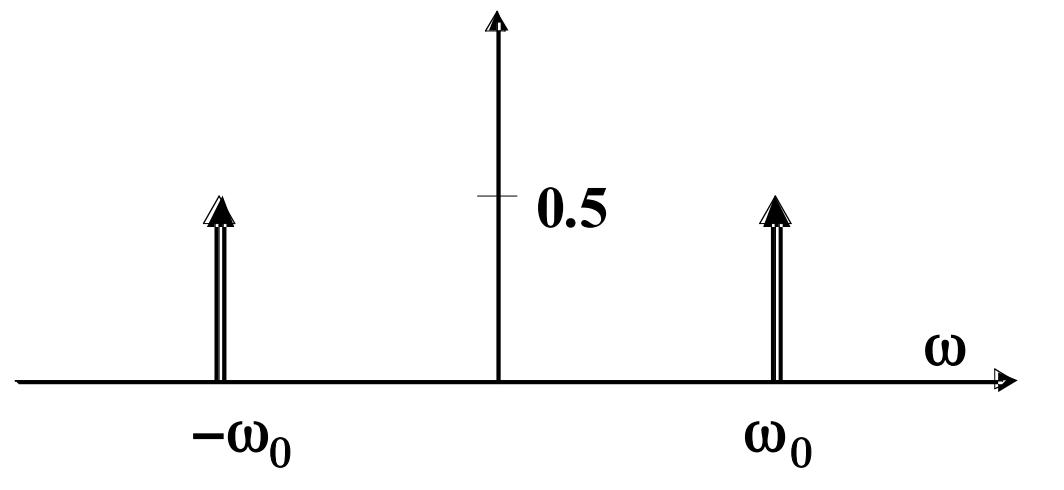
\includegraphics[width=4.5cm]{sin-mod} \caption{}
			\end{subfigure}
			\begin{subfigure}{0.48\linewidth}
				\centering
				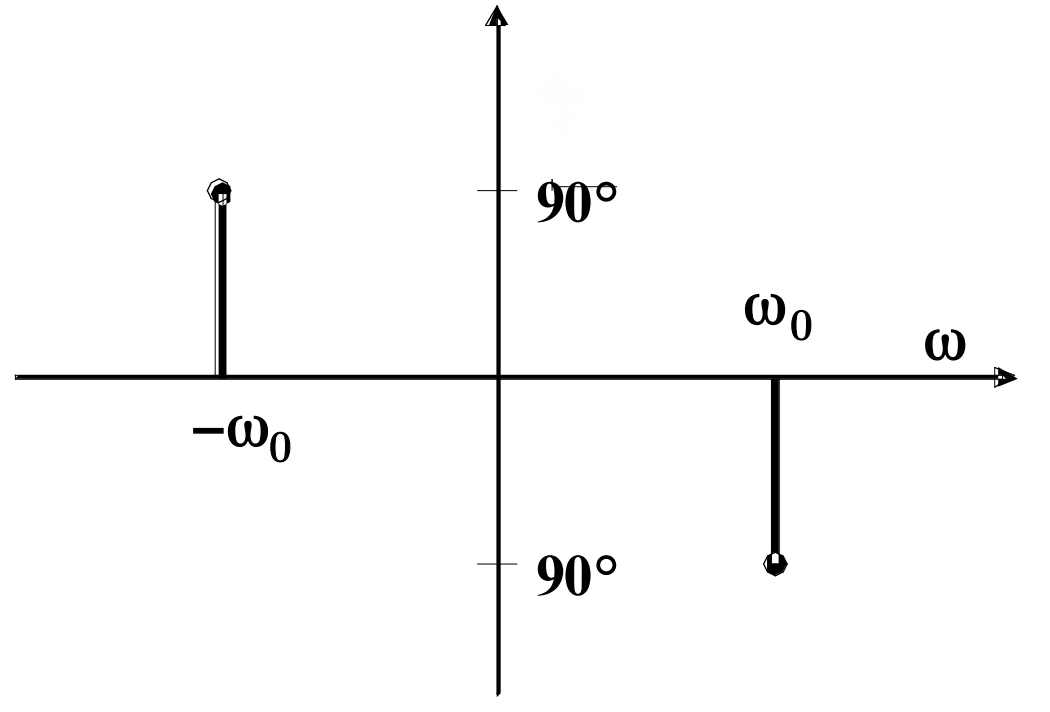
\includegraphics[width=4.5cm]{sin-ang} \caption{}
			\end{subfigure}
			\caption{modulo (a) e fase (b) dello spettro della funzione $\sin(\omega_0 t)$.}
			\label{fig:four:spettroseno}
		\end{figure}
		
		Per via della definizione della funzione $\delta$ di Dirac, scelta una qualsiasi funzione di trasferimento $H(\omega)$ risulta verificato che l'integrale in tutto lo spettro delle frequenze coincide di fatto con il valore della pulsazione della funzione $H(\omega)$ valutata nell'istante $\omega_0$ nel quale avviene l'impulso:
		\[ \int_{-\infty}^\infty H(\omega)\, \delta(\omega-\omega_0) \, d\omega = H(\omega_0)\]
		\begin{nota}
			La funzione $\delta$ moltiplica per un valore infinito il valore di $H$ nel punto $\omega_0$ (annullando il resto del dominio), tuttavia integrando in un intervallo infinitesimo $d\omega$ dello stesso ordine dell'infinito, i due termini si \textit{elidono} portando al risultato mostrato.
		\end{nota}
		
		Scomponendo la funzione di trasferimento $H$ nel suo modulo $M$ e fase $\phi$ secondo la relazione $H(\omega) = M(\omega) e^{i\phi(\omega)}$ (dove $M(\omega)$ è sempre un valore scalare!)  è possibile calcolare la risposta del sistema attraverso il prodotto della funzione di trasferimento per lo spettro del segnale sinusoidale ricavato in precedenza, arrivando al risultato
		\begin{align*}
			Y(\omega) & = H(\omega) \, U(\omega) = H(\omega) \left(\frac i 2 \delta(\omega + \omega_0) - \frac i 2 \delta(\omega-\omega_0)\right) \\
			& = H(-\omega_0) \frac i 2 \delta(\omega+\omega_0) - H(\omega_0) \frac i 2 \delta(\omega-\omega_0) \\
			& = M(\omega_0) \frac i 2 \delta(\omega+\omega_0) e^{-i\phi(\omega_0)} - M(\omega_0) \frac i 2 \delta(\omega-\omega_0) e^{i\phi(\omega_0)}
		\end{align*}
		
		Considerando le proprietà dello spettro di un segnale che permettono di affermare che il modulo $M$ è simmetrico rispetto all'asse delle ordinate, mentre la fase $\phi$ è antisimmetrica, tramite manipolazione dell'equazione di Eulero $e^{i\phi} = \cos \phi + i\sin\phi$ è possibile esprimere il rapporto tra risposta $Y$ e modulo $M$ (valutato nella pulsazione del segnale originario) come
		\begin{equation*}
			\frac{Y(\omega)}{M(\omega_0)} = \cos \big(\phi(\omega_0)\big) \underbrace{\left[ \frac i 2 \delta(\omega+\omega_0) - \frac i 2 \delta(\omega-\omega_0)\right]}_{\four{\sin(\omega_0 t)}} + \sin \big(\phi(\omega_0)\big) \underbrace{\left[ \frac 1 2 \delta(\omega+\omega_0) + \frac 1 2 \delta(\omega-\omega_0)\right]}_{\four{\cos(\omega_0 t)}}
		\end{equation*}
		
		Osservando il risultato è possibile osservare che il coefficiente di $\cos\big(\phi(\omega_0)\big)$ coincide con la trasformata della funzione iniziale $\sin(\omega_0t)$, mentre è possibile dimostrare per analogia che il coefficiente di $\sin\big(\phi(\omega_0)\big)$ è pari alla trasformata del segnale cosinusoidale di pulsazione $\omega_0$:
		\[ \cos(\omega_0 t) \quad \mapsto \quad \frac 1 2 \delta(\omega+\omega_0) + \frac 1 2 \delta(\omega-\omega_0)  \]
		Condensando i risultati ottenuti è dunque possibile antitrasformare per ottenere la risposta del sistema nel dominio del tempo con il risultato che
		\begin{equation}
		\begin{split}
			y(t) & = M(\omega_0) \cos\big(\phi(\omega_0)\big) \sin(\omega_0t) + M(\omega_0) \sin\big(\phi(\omega_0)\big) \cos(\omega_0 t) \\
			& =M(\omega_0) \sin\big(\omega_0 t + \phi(\omega_0)\big)
		\end{split}
		\end{equation}
		
		Questa relazione ci permette dunque di capire che se un sistema di equazioni differenziali lineari presenta come ingresso forzante un ingresso armonico unitario di pulsazione $\omega_0$, allora l'uscita del sistema sarà un'altra armonica di pulsazione invariata $\omega_0$ che risulterà moltiplicato e sfasato in base alle componenti della funzione di trasferimento $H$ valutata nella pulsazione $\omega_0$; un altro modo per osservare che i moduli delle funzioni $H,U$ si moltiplicano mentre le fasi si sommano si poteva ricavare considerando che
		\[Y(\omega) = H(\omega) U(\omega) = M_H(\omega) e^{i\phi_H(\omega)} + M_U(\omega) e^{i\phi_U(\omega)} = M_H(\omega)M_U(\omega) e^{i \left( \phi_H(\omega) + \phi_U(\omega) \right)}\]
	
	\subsection{\textit{Discrete Fourier Transform}}
		Nella pratica di misura attualmente si effettua un'elaborazione di segnali digitali che sono dunque discretizzati nel tempo; il segnale in ingresso al sistema di misura non sarà più dunque una funzione continua nel tempo $s(t)$, ma potrà essere considerato come una sequenza di valori $s_k$; il tempo che intercorre tra un campione e l'altro è pari al \de{periodo di campionamento} $T_c$ che coincide con l'inverso della \de{frequenza di campionamento} $f_c$.
		
		Per analizzare questo tipo di segnali si ricorre alla \de{trasformata di Fourier discreta} \textbf{DFT} (\textit{Discrete Fourier Transform}), l'analogo della trasformata di Fourier per segnali discretizzati nel tempo e che si basa anch'essa sulla scomposizione in basi ortonormali. L'algoritmo  che si occupa di trasformare segnali discreti prende il nome di \textbf{FFT} \de{\textit{Fast Fourier Transform}}.
		
		Data dunque una serie di $n$ di campioni $s_i$ discretizzati, la sequenza $Sf_n$ ottenuta dalla DFT sarà composta da un numero di elementi pari a $n$ (numero di campioni analizzati) con una risoluzione in frequenza pari a 
		\[ \Delta_f = \frac 1 {n\,T_c}\]
		La risoluzione in frequenza si può ottenere considerando che alla frequenza di campionamento $f_c$ il periodo temporale che intercorre per analizzare $n$ campioni è proprio pari a $n T_c$ e dunque la minima frequenza presente nel segnale è pari all'inverso di tale valore.
		
		In realtà per il \textbf{teorema di Nyquist} è possibile osservare che dello spettro ricavato, solo la prima meta (associato alle frequenze inferiori a $f_c/2$) ha un significato reale, in quanto i successivi valori ottenuti sono la copia ribaltata della prima parte dello spettro (dovuto alla simmetria delle componenti negative). Il valore $f_n = f_c/2$ prende dunque il nome di \de{frequenza di Nyquist} e rappresenta la frequenza limite dello spettro che si può ricavare dalla DFT.
		
		\figura{6}{1}{dft-simmetria}{esempio di DFT di un segnale; è possibile osservare la specularità dello spettro rispetto al punto medio.}{dft-simmetria}
		
		
\section{Taratura dinamica}
	\marginnote{27/04/2021}
		
		Durante la taratura statica si effettua la stima dei coefficienti di una relazione matematica (tendenzialmente polinomiale) che lega il misurando con l'uscita dello strumento in condizioni statiche. Dualmente si effettua una \de{taratura dinamica} quando si vuole stimare i coefficienti delle relazioni che governano la dinamica tra misurando e uscita dello strumento. Questo problema è strettamente legato alla risoluzione di equazioni differenziali e, ipotizzando che le stesse siano lineari, è possibile dunque risolvere il problema utilizzandola trasformata di Fourier.
		
		La taratura dinamica si occupa di determinare i parametri della funzione complessa di trasferimento $H(\omega)$ del sistema di misura nel caso in cui:
		\begin{itemize}
			\item non si conosce il modello matematico ne i parametri del sistema di misura. In questo caso è necessario determinare la funzione di trasferimento direttamente nel dominio della frequenza in quanto nessuna informazione è nota a priori;
			\item il modello matematico è noto, ma non i suoi parametri. In questo caso conoscendo l'equazione differenziale che regola la relazione ingresso-uscita è sufficiente stimare i parametri mediante delle tecniche nel dominio del tempo.
		\end{itemize}
		
	\subsection{Tecniche nel dominio della frequenza}
		\subsubsection{Ingressi armonici variabili in frequenza}
		Per effettuare la taratura è possibile imporre degli \textbf{ingressi armonici} variabili in ingresso; noto infatti l'ingresso $u(t) = \sin(\omega_0 t)$, allora l'uscita del sistema (per quanto visto dall'analisi di Fourier) dipende dalla funzione di trasferimento nel punto $\omega_0$ definita come $H(\omega_0) = M(\omega_0) e^{i\phi(\omega_0)}$ secondo la legge
		\[ y(t) = M(\omega_0 ) \sin \big(\omega_0 t+ \phi(\omega_0) \big)\]
		
		Variando il parametro $\omega_0$ è possibile misurare sia i coefficienti $M(\omega)$, sia gli sfasamenti $\phi(\omega)$ e dunque per interpolazione è possibile ricavare il modello del sistema dinamico.
		
		Il problema di questa metodologia di taratura della funzione di trasferimento è la necessità di imporre in ingresso segnali armonici puri ad una pulsazione $\omega_0$; nel caso di circuiti elettrici questo può essere fatto con una certa precisione, mentre per altri sistemi (come quelli meccanici e termici) l'operazione non può essere fatta tanto facilmente.\\
		Nel caso di sistemi meccanici in particolare si utilizzano i cosiddetti \textit{shaker}, degli agitatori  elettrodinamici che producono moti armonici di spostamento/velocità/accelerazione.
			
		\begin{nota}
			In generale non tutti i sistemi da tarare possono essere analizzati imponento un ingresso sinusoidale di frequenza nota.	
		\end{nota}
	
	\subsubsection{Rapporto delle trasformate}
		Considerato che un segnale impulsivo ideale, rappresentanto dalla funzione $\delta(t)$ delta di Dirac, presenta tutte le armoniche con impulso unitario e sfasamento nullo, è possibile determinare la funzione di trasferimento $H(\omega)$ come la risposta al sistema all'impulso:
		\[ Y(\omega) = H(\omega)\, U(\omega) \quad \xrightarrow{U(\omega) = 1 \ \forall \omega} \quad H(\omega ) = Y(\omega) \]
		Questo ci permette di capire che, tramite trasformazione della risposta $y(t)$ del sistema, è possibile stabilire la funzione di trasferimento $H(\omega)$.
		
		\vspace{3mm}
		
		Un problema legato a questo metodo di misurazione della funzione di trasferimento è che spesso, per molti sistemi, non è possibile generare un segnale impulsivo sufficientemente ideale: per questo si ricorre al determinare il rapporto delle trasformate di un segnale completamente casuale che in generale avrà modulo costante (e dunque può essere normalizzato al valore unitario) lungo tutto lo spettro.
		
		A questo punto esplicitando funzione di trasferimento e trasformata dell'ingresso nella componente di modulo e fase, è possibile osservare che
		\[ Y(\omega) = M_H(\omega) e^{i\phi_H(\omega)} M_U(\omega) e^{i\phi_U(\omega)}  \]
		Avendo ipotizzato che il modulo $M_U(\omega) = 1$ sia unitario per tutto lo spettro delle frequenze, allora è possibile riscrivere la trasformata dell'uscita dalla quale si ricava la sua relazione con il modulo della funzione di trasferimento:
		\[ Y(\omega) = M_H(\omega) e^{i\left[\phi_H(\omega) + \phi_U(\omega)\right]}  \qquad \Rightarrow \quad  M_H(\omega) = M_Y(\omega) \]
		
		In questo caso il segnale in ingresso viene denominato \textbf{rumore bianco}, in quanto è un rumore sempre presente ad ogni frequenza (derivante proprio dalla luce bianca che ha uno spettro di frequenza infinito).
		
		A livello ideale infatti sarebbe possibile pensare di determinare la funzione di trasferimento $H(\omega)$ come il rapporto tra la risposta di un sistema e il relativo ingresso cui esso era sottoposto; nella pratica tuttavia non è possibile utilizzare un segnale qualsiasi in quanto un generico ingresso $u(t)$, se trasformato, presenterà uno spettro $U(\omega)$ e relativa risposta $Y(\omega)$ con intervalli di frequenza di modulo nullo. In generale ai segnali che si rilevano è sempre sovrapposto del rumore e dunque l'antitrasformata che si misura assume valore
		\[ M_H(\omega) = \frac{M_Y(\omega) \pm \epsilon_y}{ M_U(\omega) \pm \epsilon_u } \quad \xrightarrow[M_U(\omega)\rightarrow 0]{M_Y(\omega) \rightarrow 0} \quad M_H(\omega) \approx \frac {\epsilon_y}{\epsilon_u} \]
		Si osserva dunque che l'assenza di alcune armoniche nella trasformata dell'ingresso comporta un errore nel determinare il modulo della funzione di trasferimento $M_H$.		
	
	\subsection{Tecniche nel dominio del tempo}
		
	
	
	\paragraph{Modello noto} Considerando di conoscere il modello dello strumento, per effettuare la taratura dinamica è possibile utilizzare degli ingressi canonici effettuando la taratura minimizzando gli scarti quadratici medi.
	
	Considerando per esempio una sonda \texttt{PT100} per la misura della temperatura realizzata da un filo trasduttore in platino, è possibile calcolare l'energia $E$ dello strumento posto a temperatura assoluta $T$ e il flusso di calore tra sonda e ambiente $P$ come
	\[E=mc T \qquad P = \alpha A \big(T_{amb} - T\big) \]
	Il modello matematico del problema è dato dall'equazione differenziale
	\[ \frac{dE}{dt} = P \qquad \rightarrow \quad mc \frac {dT}{dt} = \alpha A \big(T_{amb} - T \big)  \]
	Trasformando questa equazione nel dominio della frequenza tramite Fourier si ricava che
	\[ u\omega m c = \alpha A \big(T_{amb}(\omega) \omega -T(\omega)\big) \qquad T(\omega) \big(i\omega m c + \alpha a\big) = \alpha A T_{amb}(\omega)\]
	Dovendo misurare la temperatura $T_{amb}$ valutando la temperatura $T$ è possibile connotare la funzione di trasferimento come
	\[ H(\omega) = \frac 1 {1 + i\omega \frac{mc}{\alpha A}}\]
	dove $\frac{mc}{\alpha A} = \tau$ è l'unico parametro temporale del sistema che deve essere valutato tramite la taratura dinamica.
	
	Per la taratura si impone un ingresso a scalino inserendo la sonda (che stava libera all'aria) velocemente in un contenitore pieno di fluido caldo/freddo. L'inserimento che può richiedere $1/10s$ (e dunque $10Hz$) può essere considerato istantaneo se si misura che la costante di tempo $\tau$ del sistema di misura risulta valere $50s$(e dunque $0.02Hz \ll 10Hz$).
	
	Nel dominio del tempo è possibile calcolare la temperatura $T(t)$ misurata come
	\[T(t) = \big(T_{iniz} - T_{fin}\big) e^{-t/\tau} + T_{fin} \]
	Per ricavare il parametro $\tau$ del sistema è possibile ricorrere a più metodi:
	\begin{enumerate}
		\item il primo è basato sulla manipolazione dell'equazione algebrica che risolve l'equazione differenziale per l'ingresso allo scalino, in particolare si trovando la temperatura $T(\tau)$ associata al tempo $t=\tau$ si determina il valore della costante:
		\[ T(\tau) = \big(T_{iniz} - T_{fin}\big) e^{-1} + T_{fin} \]
		
		\item \textit{riscalo temperatura per renderla lineare}
	\end{enumerate}

	\paragraph{Filtraggio online e offline} Si parla di \textbf{filtraggio online} quando l'operazione di filtraggio viene effettuata ad ogni campione in ingresso (\textit{processing in real time}), mentre si parla di \textbf{filtraggio offline} quando il filtraggio viene effettuato sull'insieme di dati già acquisiti.
	
	Un filtro online discreto semplice è quello del primo ordine per il quale un ingresso $u(t)$ (e dunque $U(\omega)$) viene modificato in un'uscita $y(t)$ (analogamente $Y(\omega)$) da un fattore moltiplicativo
	\[ \frac 1 {1 + i\omega \tau} \qquad \xrightarrow{Y(\omega) = G U(\omega)} Y(\omega) + \tau i \omega Y(\omega) = U(\omega) \]
	Antitrasformando con Fourier questa relazione si ricava l'equazione differenziale che governa l'uscita
	\[y(t) + \tau \frac{dy(t)}{dt} = u(t)\]
	Discretizzando questa equazione continua (utilizzando la derivata di Eulero come approssimazione di $dy/dt$) si ottiene la funzione discretizzata
	\[ y_k + \tau \frac{y_k - y_{k-1}}{T_c} = y_k \left(1 + \frac \tau {T_c} \right) - \frac \tau {T_c} y_{k-1} = u_{k-1} \]
	\[  \Rightarrow \quad y_k = \frac{\tau / T_c}{1 + \frac{\tau}{T_c}} y_{k-1} + \frac 1  { 1+ \frac \tau {T_c}} u_{k-1} \]
	Questa successione per ricorrenza permette di capire coma lavora un filtro digitale, ossia i coefficienti $a$ e $b$ da porre prima dei valori $y_{k-1}$ e $u_{k-1}$ per calcolare $y_k$. Il problema di questo tipo di filtri è che introducono un ritardo nella misura.
	
	Uno strumento di misura dinamica ideale è quello con frequenza di taglio di molto maggiore della frequenza caratteristica del problema in quanto lascia invariato il modulo della risposta in frequenza e non introduce alcun sfasamento, tuttavia questo non sempre è possibile. Un modo per ridurre questo problema sarebbe di filtrare il segnale in uscita con un filtro inverso $H^{-1}$ che permette, teoricamente, di ripristrinare il segnale originario. Tuttavia questo metodologia non annullerebbe il rumore bianco che tenderebbe ad \textit{esplodere}. 
	
	\vspace{3mm}
	Un filtraggio offline invece non introduce degli sfasamenti ma, avendo un'istantanea di tutto il segnale campionato, è possibile attenuare delle frequenze determinate senza cambiarne la fase.
	
	
	
	
	
	\begin{esempio}{: taratura di una sonda termica}
		Si consideri una sonda \texttt{PT-100} composta da un filamento in platino posto ad una temperatura $T_s$ con massa $m_s$ e capacità termica $c_s$; la sonda è rivestita da una guaina di temperatura $T_g$, massa $m_g$ e capacità $c_g$ e lo scambio termico di coefficiente $\alpha_{gs}$ avviene tra un'area di contatto $A_{gs}$. La guaina è immessa in un un fluido a temperatura $T_m$ e la superficie di contatto pari a $A_{mg}$ con coefficiente $\alpha_{mg}$.
		
		Le equazioni differenziali che governano il problema sono dunque
		\[ m_s c_s \frac{dT_s}{dt} \alpha_{gs} A_{gs} \big(T_g -T_s\big) \qquad m_g c_g \frac{dT_g}{dt} = \alpha_{mg} A_{mg} \big(T_m-T_g\big) + \alpha_{gs}A_{gs}(T_s- T_g)\]
		
		Per calcolare la funzione di trasferimento del sistema è necessario trasformare le equazioni nel dominio delle frequenze; considerando la prima equazione si ottiene l'espressione
		\[m_s c_s i\omega T_s(\omega) = \alpha_{gs} A_{gs}\Big( T_{g}(\omega) - T_{s}(\omega)\Big) \]
		dalla quale si ricava la temperatura $T_g$ in funzione della temperatura $T_s$:
		\[ T_g(\omega) = T_s(\omega) \frac{m_s c_s i\omega + \alpha_{gs} A_{gs}}{\alpha_{gs}A_{gs}} \]
		
		Trasformando la seconda equazione differenziale nel dominio della frequenza e sostituendo il valore di $T_g$ come appena determinato è possibile determinare
		\[ m_g c_g i\omega T_g(\omega) = \alpha_{mg} A_{mg} \Big(T_m(\omega) - T_g(\omega)\Big) + \alpha_{gs} A_{gs} \Big(T_s(\omega) - T_g(\omega)\Big) \]
		\[ \Rightarrow \quad H(\omega) = \frac 1 {1 + i\omega \dfrac{m_s c_s (\alpha_{mg} A_{mg} + \alpha_{gs} A_{gs} ) + m_g c_g \alpha_{gs} A_{gs} }{\alpha_{gs} A_{gs}\alpha_{mg} A_{mg} }  + \big(i\omega\big)^2 \dfrac{m_s c_s m_g c_g}{\alpha_{gs} A_{gs} \alpha_{mg} A_{mg} } } \]
		
		Si osserva dunque che la funzione di trasferimento è del secondo ordine in quanto a denominatore contiene un termine $\omega^2$.
		
	\end{esempio}
	
	
	
	
	
	
	
	
	
	
	
	
	
	
	
	
	
	
	
	
	
	
	
	\chapter{Termocoppie e termoresistenze}
	La misura di temperatura avviene misurando la differenza di forza elettromotrice (tensione) di una termocoppia
	
	\paragraph{Effetto Peltier} Quando una corrente inizia a scorrere nella termocoppia, sui giunti metallici si genera del calore (o esso viene dissipato) in modo da controbilanciare l'effetto Seebeck, anche se spesso questo effetto viene trascurato.
	
	\paragraph{Effetto Thomson} L'effetto Thomson rileva la dispersione di calore dovuta al filo che collega le due termocoppie.
	
	In generale
	
	\[ fem_{termocoppia} = \underbrace{c_1 \big(T_1-T_2\big)}_\textrm{Seebeck} +\underbrace{ c_2\big(T_1^2-T_2^2\big)}_\textrm{Thomson}\]
	dove $c_1,c_2$ sono due costanti generalmente fornite dal produttore ma che devono essere tarate per migliorare la precisione di misura. In generale i fili di connessione delle due giunzioni possono essere esposti a temperature ambientali variabili in quanto non influiscono nella misurazione della forza elettromotrice della termocoppia.
	
	Nella pratica le termocoppie sono caratterizzate dal non avere la necessità di avere un ambiente termostatato, ma si integra il controllore con un sensore di temperatura con il quale fare il confronto di temperatura; il sistema si comporta come un termometro dunque.
	
	
\section{Termoresistenze}

	\chapter{Esperienza di laboratorio}
\section{Acceleratori allo stato solido}
	Negli smartphone sono presenti accelerometri \textit{low-cost} che si basas sulla micro-lavorazione del silicio; di per se il sensore non sarebbe \textit{buono}, tuttavia l'effetto dovuto all'elevato guadagno in retroazione si \textit{migliora} il comportamento del segnale.
	
	\textbf{SCHEMA}
	
	Osservando lo schema è possibile capire come l'accelerazione permette di spostare  il piatto centrale: questo cambia la capacità relativa tra le due armature fisse e dunque è possibile stimare il misurando. 
	
	Per migliorare la misura ci si aiuta con dell'elettronica che, tramite retroazione, tende ad evitare lo spostamento della massa centrale (e dunque la parte meccanica di \textit{scarsa qualità} associata al silicio) e dunque la stima dipende dalla misura della capacità, che può essere effettuata con buona precisione. La misura viene effettuata considerando che la forza dovuta alle armature elettriche che deve essere impressa al corpo è proporzionale all'accelerazione.
	
	
	
	\chapter{Accelerometri}
	Un \de{accelerometro} è uno strumento utilizzato per misurare l'accelerazione, rispetto ad un sistema inerziale, cui è sottoposto un corpo; per integrazione è dunque possibile stimare velocità e spostamento del corpo che si sta analizzando.
	
	E' possibile osservare che la velocità può essere analizzata sia come integrazione dell'accelerazione, sia tramite derivazione della posizione (misurata tramite encoder, per esempio):
	\[ v(t) = \int a(\xi)\, d\xi \mapsto \frac 1{i\omega} A(\omega) \qquad v(t) = \frac{dx}{dt}\mapsto i X (\omega) \]
	Osservando le relazioni è possibile osservare che la velocità ottenuta tramite integrazione dell'accelerazione di fatto moltiplica le armoniche a bassa frequenza attenuando quelle ad alta frequenza, mentre al contrario la velocità per derivazione della posizione di fatto comporta l'amplificazione delle armoniche a pulsazione elevata (eliminando quelle molto basse).
	
	Per integrazione dunque si ha l'attenuazione degli errori dovuti alle alte frequenze, mentre possono diventare importanti gli errori a frequenza elevata.
	
	
	
	
	
\section{Accelerometro a massa sismica}
	L'accelerometro a massa sismica è uno strumento che permette di misurare il moto assoluto di una massa; la risposta in frequenza di tale dispositivo comprende le frequenze pressocché nulle fino a valori molto elevate, per questo può essere utilizzato per misurare sia accelerazioni statiche che vibrazioni e/o shock.
	
	Il sistema di un accelerometro a massa sismica presenta una massa $m$ che, tramite un sistema molla-smorzatore, è collegata al grado di libertà che vuole misurare. Per misurare l'accelerazione è dunque necessario misurare lo spostamento relativo della massa all'interno del suo contenitore.
	
	\paragraph{Blocco dell'accelerometro} Considerando di imporre un'accelerazione costante $a = \ddot x$ positiva verso l'alto, allora la forza di inerzia che si oppone sulla massa è pari a $F=m\ddot x$; tale forza dovrà essere controbilanciata opportunamente da una molla la cui forza dipende dallo spostamento relativo rispetto alla posizione di riposo $F= k \, \Delta x$.
	\[ m\ddot x = k \, \Delta x \qquad \ddot x \xrightarrow{\frac m k} \Delta x\]
	
	Analizzando il sistema alle impedenze generalizzate è possibile dunque ricavare la funzione di trasferimento cui è soggetto il sistema in funzione dei parametri $m$, $k$ e $c$; per fare questo è necessario individuare i gradi di libertà associati: $B$ associato alla massa e $A$ associato alla base dello strumento. Nota la trasformata $A(\omega)$ dell'accelerazione $a(t)$ imposta alla base. Definito lo spostamento relativo $x_0 = x_A-x_B$ tra massa e base è possibile riscrivere il sistema alle impedenze generalizzate.\\
	In particolare tra i noti $A,B$ si osserva il parallelo della molla e dello smorzatore, mentre la massa $m$ è posta tra $B$ e terra; per determinare $H(\omega) = X_0(\omega) / A(\omega)$ è necessario ricondurre l'accelerazione in ingresso ad una velocità $V(\omega)$, mentre in uscita non rileviamo la posizione relativa $X_0$ ma la velocità relativa $V_0$, e dunque la funzione di trasferimento si basa sul determinare il rapporto tra $V_{AB}$ e $V_{AT}$:
	\begin{align*}
		\frac{V_{AB}(\omega)}{V_{AT}(\omega)} & = \frac{\dfrac{1}{\frac{k}{i\omega} + c}}{ \dfrac{1}{\frac{k}{i\omega} + c} + i\omega m} = \frac{1}{1 + \dfrac{k}{(i\omega)^2m} + \dfrac{c}{i\omega m}} = \frac{(i\omega)^2}{(i\omega)^2 + \dfrac k m + i\omega \dfrac c m } \\
		& = \frac{(i\omega) ^2 \dfrac m k}{1 + i\omega \dfrac c k + (i\omega)^2 \dfrac m k} \\
		H(\omega) = \frac{X_0(\omega)}{A(\omega)} & = \frac{\dfrac{1}{i\omega} V_{AB}(\omega)}{i\omega A(\omega)} = \frac{1}{(i\omega)^2} \frac{V_{AB}(\omega)}{V_{AT}(\omega)} = \frac{ m/k}{1 + i\omega \frac c k + (i\omega)^2 \frac m k}  \\
		&  = \frac{1 / \omega_n^2}{1+2\xi \dfrac{i\omega}{\omega_n} + \left(\dfrac{i\omega}{\omega_n}\right)^2 } \qquad \leftarrow \quad \omega_n = \sqrt{\frac k m}
	\end{align*}
	
	A questo punto è necessario integrare al sistema un misuratore di spostamento relativo, tramite dei sistemi di tipo estensimetrico, a potenziometro, capacitivi...
	
	
\section{Accelerometri piezo-elettrici}
	
	
	
	
	
	
	
	
	
	
	
	
	
	
	
	
	
	
	
	
%	\chapter{Esercizi d'esame}

\section{Problemi meccanici alle impedenze generalizzate}
	
	\subsection*{28 luglio 2005}
		\paragraph{Testo} Dato lo schema di un accelerometro estensimetrico in \textbf{figura}; nel sistema l'ingresso è data dall'accelerazione $a$ che è il misurando, mentre l'uscita del sistema è lo sbilanciamento $\Delta V$ del ponte di Wheatstone. 
		
		\textbf{FIGURA}
	
		All'interno della scatola del sistema è presente una massa $m = 50g$ il cui moto è smorzato (con un valore di smorzamento $c_{eq} = 0.2 kg/s$) da un bagno d'olio che circonda il sistema. Il principio di misura si basa sulla misura di deformazione (con coefficiente elastico $k_{eq} = 10kN/m$) della mensola su cui si poggia la massa in funzione dell'accelerazione applicata.
		
		\paragraph{Risoluzione} Imponendo al sistema di misura un'accelerazione $a$ positiva, allora la massa per il terzo principio della dinamica spingerà \textit{verso il basso} con una forza $F = ma$: questo porta ad una deflessione \textit{a S} della mensola di appoggio.
		
		Supponendo di aver posto 2 estensimetri per ogni estremità della mensola dove si attacca con la base, allora l'estensimetro superiore tenderà ad allungarsi (aumento di resistenza), mentre quello inferiore tenderà a contrarsi (diminuzione di resistenza)
		
		
		
		
		
	
\end{document}